% ============================================================================
% 甄嬛传·千声千面 —— AI 角色语音对话系统
% 终期论文
% ============================================================================
% 成员A: 李思婷 2023212061 — 数据处理与CosyVoice模型训练
% 成员B: 张笑   2023212062 — GPT-SoVITS微调与ASR+LLM对话模块
% 成员C: 黄艺平 2023212179 — 前端设计与系统集成
% ============================================================================

\documentclass[12pt,a4paper]{article}

% ── 中文支持 ──────────────────────────────────────────────────────────────
\usepackage[UTF8,fontset=none]{ctex}
\setCJKmainfont{SimSun}[AutoFakeBold=2.5,AutoFakeSlant=0.2]
\setCJKsansfont{SimHei}[AutoFakeBold=2.5]
\setCJKmonofont{KaiTi}
\newCJKfontfamily\heiti{SimHei}[AutoFakeBold=2.5]
\setmainfont{Times New Roman}

% ── 页面布局 ──────────────────────────────────────────────────────────────
\usepackage[left=2.5cm, right=2.5cm, top=2.5cm, bottom=2.5cm]{geometry}
\usepackage{setspace}
\onehalfspacing
\setlength{\hfuzz}{25pt}
\hbadness=10000

% ── 图表与代码 ────────────────────────────────────────────────────────────
\usepackage{graphicx}
\usepackage{float}
\usepackage{booktabs}
\usepackage{longtable}
\usepackage{multirow}
\usepackage{array}
\usepackage{tabularx}
\usepackage{caption}
\usepackage{subcaption}
\counterwithout{figure}{section}
\counterwithout{table}{section}
\usepackage{listings}
\usepackage[table]{xcolor}

% ── 代码样式 ──────────────────────────────────────────────────────────────
\lstset{
    basicstyle=\small\ttfamily,
    breaklines=true,
    frame=single,
    backgroundcolor=\color{gray!5},
    rulecolor=\color{gray!40},
    numbers=left,
    numberstyle=\tiny\color{gray},
    keywordstyle=\color{blue!70},
    commentstyle=\color{green!50!black},
    stringstyle=\color{red!60},
    showstringspaces=false,
    tabsize=4
}

% ── 链接与引用 ────────────────────────────────────────────────────────────
\usepackage[colorlinks=true,
            linkcolor=blue,
            citecolor=blue,
            urlcolor=blue]{hyperref}

% ── 数学与符号 ────────────────────────────────────────────────────────────
\usepackage{amsmath,amssymb}
\usepackage{enumitem}

% ── TikZ 流程图 ────────────────────────────────────────────────────────────
\usepackage{tikz}
\usetikzlibrary{
    shapes.geometric,
    arrows.meta,
    positioning,
    fit,
    backgrounds,
    calc
}
% 成员A专属配色（蓝色系——李思婷：数据处理与CosyVoice）
\definecolor{Alight}{RGB}{214, 234, 248}
\definecolor{Amid}{RGB}{41, 128, 185}
\definecolor{Adark}{RGB}{27, 79, 114}
\definecolor{Agray}{RGB}{235, 242, 250}
% 成员B专属配色（绿色系——张笑：GPT-SoVITS与ASR+LLM）
\definecolor{Blight}{RGB}{220, 245, 225}
\definecolor{Bmid}{RGB}{39, 174, 96}
\definecolor{Bdark}{RGB}{25, 120, 65}
\definecolor{Bgray}{RGB}{245, 247, 245}
% 成员C专属配色（红色系——黄艺平：前端设计与系统集成）
\definecolor{Clight}{RGB}{253, 236, 234}
\definecolor{Cmid}{RGB}{192, 57, 43}
\definecolor{Cdark}{RGB}{145, 35, 28}
\definecolor{Cgray}{RGB}{253, 248, 247}
% 成员A流程图样式（蓝色系）
\tikzset{
    aproc/.style={
        rectangle, rounded corners=6pt, draw=Amid, line width=1.0pt,
        fill=white, text=black, minimum width=2.6cm, minimum height=0.9cm,
        align=center, font=\footnotesize\sffamily, inner sep=6pt
    },
    aterm/.style={
        rectangle, rounded corners=8pt, draw=Adark, line width=1.2pt,
        fill=Amid, text=white, minimum width=2.6cm, minimum height=0.95cm,
        align=center, font=\footnotesize\bfseries\sffamily, inner sep=6pt
    },
    aarr/.style={-{Stealth[length=7pt, width=5pt]}, line width=0.9pt, Adark},
}
% 成员B流程图样式（绿色系）
\tikzset{
    bproc/.style={
        rectangle, rounded corners=6pt, draw=Bmid, line width=1.0pt,
        fill=white, text=black, minimum width=2.6cm, minimum height=0.9cm,
        align=center, font=\footnotesize\sffamily, inner sep=6pt
    },
    bterm/.style={
        rectangle, rounded corners=8pt, draw=Bdark, line width=1.2pt,
        fill=Bmid, text=white, minimum width=2.6cm, minimum height=0.95cm,
        align=center, font=\footnotesize\bfseries\sffamily, inner sep=6pt
    },
    barr/.style={-{Stealth[length=7pt, width=5pt]}, line width=0.9pt, Bdark},
}
% 成员C流程图样式（红色系）
\tikzset{
    cproc/.style={
        rectangle, rounded corners=6pt, draw=Cmid, line width=1.0pt,
        fill=white, text=black, minimum width=2.6cm, minimum height=0.9cm,
        align=center, font=\footnotesize\sffamily, inner sep=6pt
    },
    cterm/.style={
        rectangle, rounded corners=8pt, draw=Cdark, line width=1.2pt,
        fill=Cmid, text=white, minimum width=2.6cm, minimum height=0.95cm,
        align=center, font=\footnotesize\bfseries\sffamily, inner sep=6pt
    },
    carr/.style={-{Stealth[length=7pt, width=5pt]}, line width=0.9pt, Cdark},
}

% ── 页眉页脚 ──────────────────────────────────────────────────────────────
\usepackage{fancyhdr}
\setlength{\headheight}{14.5pt}
\pagestyle{fancy}
\fancyhf{}
\fancyhead[L]{甄嬛传·千声千面 —— AI 角色语音对话系统}
\fancyhead[R]{终期论文}
\fancyfoot[C]{\thepage}
\renewcommand{\headrulewidth}{0.4pt}


% ══════════════════════════════════════════════════════════════════════════
\begin{document}

% ── 封面页 ────────────────────────────────────────────────────────────────
\begin{titlepage}
\thispagestyle{empty}

\vspace*{1.5cm}

\begin{center}

\includegraphics[width=0.55\textwidth]{北邮校名校徽编排 横版中英文.png}
\end{center}

\vspace{1.8cm}

\begin{center}
{\Large\heiti ——\; 语音信息处理大作业 \;\textbullet\; 终期论文 \;——}
\end{center}

\vspace{2.5cm}

\begin{center}
{\fontsize{28pt}{36pt}\selectfont\heiti
甄嬛传·千声千面\\[10pt]
AI 角色语音对话系统}
\end{center}

\vspace{3.5cm}

\begin{center}
{\large
\renewcommand{\arraystretch}{1.6}
\begin{tabular}{rll}
    \textbf{成员A} & \textbf{李思婷} & 2023212061 \\
    \textbf{成员B} & \textbf{张笑}   & 2023212062 \\
    \textbf{成员C} & \textbf{黄艺平} & 2023212179 \\
\end{tabular}
}
\end{center}

\vfill

\begin{center}
{\large 2026 年 6 月}
\end{center}

\vspace{1cm}

\end{titlepage}

% ── 摘要 ──────────────────────────────────────────────────────────────────
\newpage
\pagenumbering{Roman}

\begin{center}
{\LARGE\heiti 摘\quad 要}
\end{center}
\vspace{0.5cm}

本文介绍了一个面向电视剧《甄嬛传》的 AI 角色语音对话系统------\,\textbf{甄嬛传\,\textperiodcentered\,千声千面}。该系统从 76 集原剧音频中自主构建了包含 14 个角色、13,605 段语音片段（总时长约 16.7 小时）的高质量中文语音数据集，并基于 CosyVoice3-0.5B（Zero-shot 语音克隆）和 GPT-SoVITS（微调语音合成）双引擎实现了多角色语音克隆与情感语音合成。系统结合大语言模型（LLM）实现角色性格建模与对话生成，支持单人智能对话与双人即兴对戏两种交互模式，并通过 SSE 流式传输与 Web Audio API 实现了低延迟的语音播放体验。实验表明，CosyVoice3 Zero-shot 方案在音色还原度和自然度上显著优于微调方案，创新性的\textbf{情绪 Speaker}方案有效解决了情绪控制与音色保真之间的矛盾。

\vspace{0.8cm}
\noindent\textbf{关键词：}语音克隆；语音合成；CosyVoice；GPT-SoVITS；大语言模型；说话人识别；情感语音合成

% ── 目录 ──────────────────────────────────────────────────────────────────
\newpage
\tableofcontents
\newpage
\pagenumbering{arabic}
\setcounter{page}{1}

% ══════════════════════════════════════════════════════════════════════════
\section{选题背景}
\label{sec:background}

\subsection{研究背景}

语音合成（Text-to-Speech, TTS）与语音克隆（Voice Cloning）技术在近年来取得了飞速发展。以 VALL-E、CosyVoice、GPT-SoVITS 等为代表的新一代语音合成模型，凭借强大的零样本（Zero-shot）学习能力和细粒度的韵律控制，使得高质量的个性化语音合成成为可能。与此同时，大语言模型（LLM）在自然语言理解与生成方面的突破，为构建具有角色个性的智能对话系统提供了新思路。

影视IP的语音交互应用是上述技术的典型落地场景。《甄嬛传》作为中国最具影响力的古装电视剧之一，拥有大量经典角色和丰富的台词素材，其角色声音具有高辨识度和情感表现力，是语音克隆技术的理想实验对象。然而，将语音克隆技术应用于多角色场景面临若干挑战：首先，从原始音频中提取并标注多角色数据需要完整的音频处理流水线；其次，多角色联合训练容易因数据不均衡导致过拟合；最后，在保持音色保真的同时实现情绪控制是一个尚未充分解决的问题。

\subsection{课程要求}

本项目为\textbf{语音信息处理}课程大作业，要求涵盖语音合成、语音克隆、说话人识别、情感识别等核心技术，具备完整的算法实现、自主构建数据集的能力，并展示创新应用场景。

% ══════════════════════════════════════════════════════════════════════════
\section{实验目标}
\label{sec:objectives}

本项目旨在构建一个面向《甄嬛传》的 AI 角色语音对话系统，实现以下核心目标：

\begin{enumerate}[leftmargin=*]
    \item \textbf{自主构建多角色语音数据集}：从 76 集原剧音频出发，通过人声分离、语音识别、声纹聚类与人工标注，构建包含 14 个角色的高质量中文语音数据集。
    \item \textbf{多角色语音克隆与合成}：基于 CosyVoice3-0.5B（Zero-shot）和 GPT-SoVITS（微调）双引擎实现角色声音的高保真复现，支持用户实时对比两种引擎的合成效果。
    \item \textbf{情感语音合成}：实现喜悦、愤怒、悲伤、平静四种情绪的语音合成，在不损失音色保真度的前提下自然表达角色情感。
    \item \textbf{角色智能对话}：结合 LLM 实现角色性格建模，支持\textbf{现代来客}和\textbf{宫廷中人}两种身份的单人对话，以及双角色自动即兴对戏。
    \item \textbf{完整系统集成}：构建包含 React 前端、FastAPI 后端中间层、云端 TTS/ASR/LLM 服务的完整系统，实现流式语音播放和实时交互。
\end{enumerate}

% ══════════════════════════════════════════════════════════════════════════
\section{方法流程}
\label{sec:methods}

本节详细介绍系统各模块的技术方案与实现细节。

% TODO: 后续可插入系统整体架构图
% \begin{figure}[H]
% \centering
% \includegraphics[width=0.95\textwidth]{figures/system_architecture.png}
% \caption{系统整体架构图}
% \label{fig:system-arch}
% \end{figure}

% ── 3.1 数据集构建 ────────────────────────────────────────────────────────
\subsection{数据集构建}
\label{sec:data}

\subsubsection{数据来源与规模}

本项目的数据源为电视剧《甄嬛传》全集 76 集 MP3 音频（128 kbps、44.1 kHz、立体声），已完成去片头片尾处理（无人播剧版），原始总时长约 80 小时。所有数据处理与模型训练均在 AutoDL 云 GPU 实例（RTX 4080 SUPER 单卡，16 GB 显存）上完成。

\subsubsection{数据处理 Pipeline}

从原始音频到最终数据集的完整处理流程如图~\ref{fig:data-pipeline}所示，共分为五个阶段。

\begin{figure}[H]
\centering
\begin{tikzpicture}[node distance=1.2cm, auto, scale=0.85, every node/.style={transform shape}]

    % ── 阶段节点（纵向排列）──────────────────────────────
    \node [aterm, minimum width=6.0cm]
        (s1) {\textbf{阶段一：原始数据采集} \\ {\footnotesize 76 集 MP3，44.1kHz Stereo，约 80 小时}};

    \node [aproc, below=of s1, minimum width=6.0cm]
        (s2) {\textbf{阶段二：UVR5 人声分离} \\ {\footnotesize demucs + mdx\_extra\_q $\to$ 纯净人声}};

    \node [aproc, below=of s2, minimum width=6.0cm]
        (s3) {\textbf{阶段三：VAD 切分 + ASR 转写} \\ {\footnotesize FunASR SeacoParaformer $\to$ 15,685 段 WAV（16kHz Mono）}};

    \node [aproc, below=of s3, minimum width=6.0cm]
        (s4) {\textbf{阶段四：声纹提取 + 说话人聚类} \\ {\footnotesize eres2netv2（512维）+ KMeans（$n=30$）$\to$ 30 个匿名簇}};

    \node [aproc, below=of s4, minimum width=6.0cm]
        (s5) {\textbf{阶段五：人工标注 + 数据清洗} \\ {\footnotesize 每簇抽 5 条试听，三轮迭代 + 4 轮过滤 $\to$ 14 角色}};

    \node [aterm, below=of s5, minimum width=6.0cm]
        (s6) {\textbf{最终数据集} \\ {\footnotesize 14 角色 $\cdot$ 13,605 段 $\cdot$ 约 1,005 分钟（16.7 小时）}};

    % ── 箭头 ────────────────────────────────────────────
    \draw [aarr] (s1) -- (s2);
    \draw [aarr] (s2) -- (s3);
    \draw [aarr] (s3) -- (s4);
    \draw [aarr] (s4) -- (s5);
    \draw [aarr] (s5) -- (s6);

    % ── 右侧产出标注 ────────────────────────────────────
    \node [font=\footnotesize\color{Adark}, anchor=west, align=left, xshift=8pt]
        at (s2.east) {$\to$ 纯净人声 44.1kHz Stereo};
    \node [font=\footnotesize\color{Adark}, anchor=west, align=left, xshift=8pt]
        at (s3.east) {$\to$ 15,685 段（2--15s/段）};
    \node [font=\footnotesize\color{Adark}, anchor=west, align=left, xshift=8pt]
        at (s4.east) {$\to$ 30 个匿名簇（spk\_00--spk\_29）};
    \node [font=\footnotesize\color{Adark}, anchor=west, align=left, xshift=8pt]
        at (s5.east) {$\to$ 15,685 $\to$ 13,605 段};

\end{tikzpicture}
\caption{数据处理 Pipeline 流程图}
\label{fig:data-pipeline}
\end{figure}

{\color{Amid}\rule{4pt}{0pt}}\,\textbf{\color{Amid}阶段一：原始数据采集}\\[3pt]
数据来自电视剧《甄嬛传》全部 76 集原声 MP3 文件。音频格式为 44.1 kHz 立体声、128 kbps 比特率，已预先去除每集的片头片尾部分（即无人播剧版本），总计时长约 80 小时。

{\color{Amid}\rule{4pt}{0pt}}\,\textbf{\color{Amid}阶段二：UVR5 人声分离}\\[3pt]
使用 UVR5\cite{uvr5} 的 demucs\cite{defossez2021demucs} 引擎配合 mdx\_extra\_q 预训练权重，对 76 集音频逐一进行人声与背景音乐的分离。该模型在音乐分离基准上对人声轨的分离效果表现优异，尤其对中文语音的中频段保留较为完整。分离后保留纯净人声轨，仍为 44.1 kHz 立体声格式，同时去除了背景音乐、环境音效等非人声成分。

{\color{Amid}\rule{4pt}{0pt}}\,\textbf{\color{Amid}阶段三：VAD 切分 + ASR 转写}\\[3pt]
采用 FunASR\cite{funasr} 的 SeacoParaformer 模型（VAD 与 ASR 二合一）对纯净人声进行语音活动检测（Voice Activity Detection）和自动语音识别（Automatic Speech Recognition）。模型首先检测音频中的语音活动区域，然后将字级别的时间戳合并为句子级片段：当相邻两句话的间隔超过 800 ms 时进行切分，确保每段 WAV 对应一句完整的台词。输出规格为 16 kHz 单声道 WAV，每段时长控制在 2$\sim$ 15 秒之间。本阶段共产生 15,685 段语音片段。

{\color{Amid}\rule{4pt}{0pt}}\,\textbf{\color{Amid}阶段四：声纹提取 + 说话人聚类}\\[3pt]
使用 3D-Speaker\cite{3d-speaker} 中的 eres2netv2 模型对全部 15,685 段 WAV 逐一提取 512 维说话人声纹特征向量（Speaker Embedding），随后使用 scikit-learn\cite{sklearn} 的 KMeans 算法（设置 $n_\text{clusters}=30$）将相似声纹特征的片段自动归入同一簇。聚类结果为 30 个匿名说话人簇（编号 spk\_00 $\sim$  spk\_29）。聚类后片段数最多的 15 个簇的分布如表~\ref{tab:cluster-top15}所示。

\begin{table}[H]
\centering
\caption{KMeans 聚类结果 Top 15（$n=30$，按片段数降序）}
\label{tab:cluster-top15}
\begin{tabular}{cccc}
\toprule
\textbf{聚类簇} & \textbf{片段数} & \textbf{时长（min）} & \textbf{人工标注映射角色} \\
\midrule
spk\_06 & 1,241 & 77.0 & 皇上·爱新觉罗·胤禛 \\
spk\_22 & 1,220 & 90.8 & 甄嬛 \\
spk\_10 & 877  & 61.6 & 甄嬛 \\
spk\_12 & 862  & 51.1 & 甄嬛 \\
spk\_14 & 754  & 58.5 & 甄嬛 \\
spk\_13 & 752  & 69.8 & 乌拉那拉·宜修（皇后） \\
spk\_21 & 747  & 54.9 & 甄嬛 \\
spk\_20 & 673  & 52.2 & 华妃·年世兰 \\
\rowcolor{red!15} spk\_25 & 666  & 60.7 & \textbf{已淘汰}（簇内混入多人声音） \\
spk\_02 & 630  & 62.6 & 皇上·爱新觉罗·胤禛 \\
spk\_18 & 623  & 41.3 & 皇上·爱新觉罗·胤禛 \\
spk\_16 & 572  & 45.3 & 崔槿汐 \\
spk\_23 & 563  & 49.5 & 沈眉庄 \\
spk\_07 & 538  & 43.0 & 安陵容 \\
spk\_29 & 528  & 47.8 & 叶澜依 \\
\bottomrule
\multicolumn{4}{p{0.95\textwidth}}{\footnotesize 注：30 个簇中，24 个成功映射到 14 个具体角色，6 个簇（spk\_00、01、05、25、26、28）为最终未被映射。其中 spk\_25（666 段）在人工标注阶段一度被识别为特定角色，但经验证发现簇内混入了多个不同说话人的声音（KMeans 错误合并），故最终淘汰。同一角色（如甄嬛）分散在多个簇中，后期人工标注环节完成跨簇合并。} \\
\end{tabular}
\end{table}

{\color{Amid}\rule{4pt}{0pt}}\,\textbf{\color{Amid}阶段五：人工标注 + 数据清洗}\\[3pt]
聚类完成后，从每个说话人簇中随机抽取 5 条音频，由人工逐一试听并根据台词内容、语气特征与剧中角色的说话风格进行综合判断，将匿名簇映射到具体角色。标注过程共经历三轮迭代交叉验证：第一轮成功映射 22/30 簇，第二轮推进至 27/30，第三轮交叉验证并纠正误标后最终确认 24/30 簇。另有 3 个簇（阿晋、净白师太、齐妃）因 KMeans 聚类不准确，簇内混入了多个不同说话人的片段，音色杂乱不可靠，经人工确认后淘汰；剩余簇为空或纯噪声。最终保留 14 个高可信度角色。

标注完成后，进行四轮数据清洗与质量过滤，各步骤过滤效果如表~\ref{tab:data-clean}所示。

\begin{table}[H]
\centering
\caption{数据清洗各步骤过滤效果}
\label{tab:data-clean}
\begin{tabular}{lccc}
\toprule
\textbf{过滤步骤} & \textbf{段数变化} & \textbf{丢弃量} & \textbf{保留率} \\
\midrule
角色过滤（去除非目标角色）         & 15,685 $\to$ 14,003 & $-$1,682 & 89.3\% \\
文本过滤（空/过短$<$2字/过长$>$80字） & 14,003 $\to$ 13,644 & $-$359  & 97.4\% \\
文本去重（完全相同台词仅保留一条）     & 13,644 $\to$ 13,613 & $-$31   & 99.8\% \\
音频质检（RMS$<$0.003静音/削波率$>$10\%） & 13,613 $\to$ 13,605 & $-$8    & 99.9\% \\
\midrule
\rowcolor{Amid!20}
\textbf{合计} & \textbf{15,685 $\to$ 13,605} & \textbf{$-$2,080} & \textbf{86.7\%} \\
\bottomrule
\end{tabular}
\end{table}

\subsubsection{最终数据集统计}

经过上述全流程处理后，最终数据集包含 14 个角色、共 13,605 段语音片段，总时长约 1,005 分钟（16.7 小时）。各角色的数据分布如表~\ref{tab:data-dist}所示。

\begin{table}[H]
\centering
\caption{14 角色数据分布}
\label{tab:data-dist}
\begin{tabular}{cccc}
\toprule
\textbf{角色} & \textbf{片段数} & \textbf{时长（min）} & \textbf{占比} \\
\midrule
\rowcolor{Amid!15} 甄嬛                         & 4,340 & 296.2 & \textbf{29.5\%} \\
\rowcolor{Amid!10} 皇上·爱新觉罗·胤禛             & 2,461 & 173.7 & \textbf{17.3\%} \\
\rowcolor{Amid!5}  乌拉那拉·宜修（皇后）           & 1,286 & 106.5 & \textbf{10.6\%} \\
崔槿汐                       & 831   & 66.3  & 6.6\%  \\
华妃·年世兰                   & 661   & 49.4  & 4.9\%  \\
沈眉庄                       & 542   & 44.9  & 4.5\%  \\
苏培盛                       & 533   & 47.5  & 4.7\%  \\
安陵容                       & 526   & 40.4  & 4.0\%  \\
叶澜依                       & 483   & 39.0  & 3.9\%  \\
浣碧                         & 477   & 36.9  & 3.7\%  \\
果郡王·允礼                   & 388   & 26.5  & 2.6\%  \\
太后                         & 516   & 35.5  & 3.5\%  \\
曹贵人                       & 308   & 27.9  & 2.8\%  \\
温实初                       & 253   & 20.0  & 2.0\%  \\
\midrule
\textbf{合计}                 & \textbf{13,605} & \textbf{$\sim$ 1,005} & \textbf{100\%} \\
\bottomrule
\end{tabular}
\end{table}

\begin{figure}[H]
\centering
\begin{tikzpicture}[scale=1.0]

% Colors for pie (dark blue → light blue gradient)
\definecolor{q1}{HTML}{0B3D5C}   \definecolor{q2}{HTML}{14527A}
\definecolor{q3}{HTML}{1B6798}   \definecolor{q4}{HTML}{247DB5}
\definecolor{q5}{HTML}{2E93D0}   \definecolor{q6}{HTML}{43A5E0}
\definecolor{q7}{HTML}{5CB5E8}   \definecolor{q8}{HTML}{78C5F0}
\definecolor{q9}{HTML}{94D2F5}   \definecolor{q10}{HTML}{ADE0F8}
\definecolor{q11}{HTML}{C2E7FA}  \definecolor{q12}{HTML}{D6EFFC}
\definecolor{q13}{HTML}{E5F4FD}  \definecolor{q14}{HTML}{F0F8FE}

\def\R{2.2}  % radius

% Draw sectors: counter-clockwise, 1%=3.6deg
\filldraw[q1]  (0,0) -- (0:\R)       arc (0:-106.2:\R)        -- cycle;  % 甄嬛 29.5%
\filldraw[q2]  (0,0) -- (-106.2:\R)  arc (-106.2:-168.5:\R)   -- cycle;  % 皇上 17.3%
\filldraw[q3]  (0,0) -- (-168.5:\R)  arc (-168.5:-206.7:\R)   -- cycle;  % 皇后 10.6%
\filldraw[q4]  (0,0) -- (-206.7:\R)  arc (-206.7:-230.5:\R)   -- cycle;  % 崔槿汐 6.6%
\filldraw[q5]  (0,0) -- (-230.5:\R)  arc (-230.5:-248.1:\R)   -- cycle;  % 华妃 4.9%
\filldraw[q6]  (0,0) -- (-248.1:\R)  arc (-248.1:-265.0:\R)   -- cycle;  % 苏培盛 4.7%
\filldraw[q7]  (0,0) -- (-265.0:\R)  arc (-265.0:-281.2:\R)   -- cycle;  % 沈眉庄 4.5%
\filldraw[q8]  (0,0) -- (-281.2:\R)  arc (-281.2:-295.6:\R)   -- cycle;  % 安陵容 4.0%
\filldraw[q9]  (0,0) -- (-295.6:\R)  arc (-295.6:-309.6:\R)   -- cycle;  % 叶澜依 3.9%
\filldraw[q10] (0,0) -- (-309.6:\R)  arc (-309.6:-322.9:\R)   -- cycle;  % 浣碧 3.7%
\filldraw[q11] (0,0) -- (-322.9:\R)  arc (-322.9:-335.5:\R)   -- cycle;  % 太后 3.5%
\filldraw[q12] (0,0) -- (-335.5:\R)  arc (-335.5:-345.6:\R)   -- cycle;  % 曹贵人 2.8%
\filldraw[q13] (0,0) -- (-345.6:\R)  arc (-345.6:-355.0:\R)   -- cycle;  % 果郡王 2.6%
\filldraw[q14] (0,0) -- (-355.0:\R)  arc (-355.0:-362.2:\R)   -- cycle;  % 温实初 2.0%

% Donut center
\fill[white] (0,0) circle (0.9);
\node[font=\footnotesize\bfseries] at (0,0) {14 角色};

% Legend ── explicit boxes (no foreach)
\begin{scope}[xshift=4.8cm, yshift=2.8cm]
\def\dy{0.40}
\filldraw[q1]  (0,0)       rectangle (0.35,0.30);  \node[anchor=west,font=\footnotesize] at (0.50,0.15) {甄嬛\quad 29.5\%};
\filldraw[q2]  (0,-\dy)    rectangle (0.35,-\dy+0.30); \node[anchor=west,font=\footnotesize] at (0.50,-\dy+0.15) {皇上\quad 17.3\%};
\filldraw[q3]  (0,-2*\dy)  rectangle (0.35,-2*\dy+0.30); \node[anchor=west,font=\footnotesize] at (0.50,-2*\dy+0.15) {皇后\quad 10.6\%};
\filldraw[q4]  (0,-3*\dy)  rectangle (0.35,-3*\dy+0.30); \node[anchor=west,font=\footnotesize] at (0.50,-3*\dy+0.15) {崔槿汐\quad 6.6\%};
\filldraw[q5]  (0,-4*\dy)  rectangle (0.35,-4*\dy+0.30); \node[anchor=west,font=\footnotesize] at (0.50,-4*\dy+0.15) {华妃\quad 4.9\%};
\filldraw[q6]  (0,-5*\dy)  rectangle (0.35,-5*\dy+0.30); \node[anchor=west,font=\footnotesize] at (0.50,-5*\dy+0.15) {苏培盛\quad 4.7\%};
\filldraw[q7]  (0,-6*\dy)  rectangle (0.35,-6*\dy+0.30); \node[anchor=west,font=\footnotesize] at (0.50,-6*\dy+0.15) {沈眉庄\quad 4.5\%};
\filldraw[q8]  (0,-7*\dy)  rectangle (0.35,-7*\dy+0.30); \node[anchor=west,font=\footnotesize] at (0.50,-7*\dy+0.15) {安陵容\quad 4.0\%};
\filldraw[q9]  (0,-8*\dy)  rectangle (0.35,-8*\dy+0.30); \node[anchor=west,font=\footnotesize] at (0.50,-8*\dy+0.15) {叶澜依\quad 3.9\%};
\filldraw[q10] (0,-9*\dy)  rectangle (0.35,-9*\dy+0.30); \node[anchor=west,font=\footnotesize] at (0.50,-9*\dy+0.15) {浣碧\quad 3.7\%};
\filldraw[q11] (0,-10*\dy) rectangle (0.35,-10*\dy+0.30); \node[anchor=west,font=\footnotesize] at (0.50,-10*\dy+0.15) {太后\quad 3.5\%};
\filldraw[q12] (0,-11*\dy) rectangle (0.35,-11*\dy+0.30); \node[anchor=west,font=\footnotesize] at (0.50,-11*\dy+0.15) {曹贵人\quad 2.8\%};
\filldraw[q13] (0,-12*\dy) rectangle (0.35,-12*\dy+0.30); \node[anchor=west,font=\footnotesize] at (0.50,-12*\dy+0.15) {果郡王\quad 2.6\%};
\filldraw[q14] (0,-13*\dy) rectangle (0.35,-13*\dy+0.30); \node[anchor=west,font=\footnotesize] at (0.50,-13*\dy+0.15) {温实初\quad 2.0\%};

\node[font=\footnotesize\color{Adark}, anchor=west] at (0.50,-14*\dy+0.15) {$\triangleright$ 甄嬛一人（29.5\%）$>$ 后 8 位小角色之和};
\end{scope}

\end{tikzpicture}
\caption{14 角色数据分布饼图}
\label{fig:pie-dist}
\end{figure}

\begin{center}
\fcolorbox{Amid}{Agray}{%
\begin{minipage}{0.92\textwidth}
\centering
\textbf{甄嬛一人（29.5\%，4,340 段）$>$ 后 8 位小角色之和} \\
数据极度不均衡是后续 CosyVoice3 全参数微调出现严重过拟合的根本原因
\end{minipage}}
\end{center}

数据集按 95:5 的比例随机划分为训练集（12,925 段）和验证集（680 段），导出为 CosyVoice Kaldi 格式（包含 wav.scp、text、utt2spk、spk2utt 及 instruct 语气指令文件），并进一步通过 CosyVoice3 内置的 campplus ONNX 和 speech\_tokenizer\_v3 ONNX 提取持续表征，输出为 Parquet 格式供训练加载。

% ── 3.2 CosyVoice3 语音克隆 ──────────────────────────────────────────────
\subsection{CosyVoice3 语音克隆}
\label{sec:cosyvoice}

\subsubsection{CosyVoice3-0.5B 微调实验}

为探索全参数监督微调（Supervised Fine-Tuning, SFT）在有限数据条件下的表现，首先对 CosyVoice3-0.5B\cite{du2025cosyvoice3} 进行了 14 角色联合微调实验。实验配置如表~\ref{tab:sft-config}所示。

\begin{table}[H]
\centering
\caption{CosyVoice3-0.5B SFT 微调配置}
\label{tab:sft-config}
\begin{tabular}{ll}
\toprule
\textbf{参数} & \textbf{值} \\
\midrule
预训练模型       & Fun-CosyVoice3-0.5B（ModelScope） \\
GPU             & RTX 4080 SUPER $\times$1, 16 GB VRAM \\
学习率           & $1 \times 10^{-5}$（预训练 lr 的 1/100） \\
学习率调度器      & ConstantLR \\
最大 Epoch       & 20（实际跑 5 轮后停止） \\
Batch Size       & 800 frames（梯度累积 $\times$2） \\
混合精度         & AMP（启用） \\
训练数据         & 12,925 条（14 角色，95\% 训练集） \\
验证数据         & 680 条（5\% 验证集） \\
微调模块         & 仅 LLM（Flow Matching 与 HiFiGAN 冻结） \\
\bottomrule
\end{tabular}
\end{table}

训练过程中记录了每个 Epoch 结束时的训练损失（Train Loss）、训练准确率（Train Acc）、验证损失（CV Loss）和验证准确率（CV Acc），如表~\ref{tab:sft-loss}所示。

\begin{table}[H]
\centering
\caption{CosyVoice3-0.5B SFT 训练过程记录}
\label{tab:sft-loss}
\begin{tabular}{ccccc}
\toprule
\textbf{Epoch} & \textbf{Train Loss} & \textbf{Train Acc} & \textbf{CV Loss} & \textbf{CV Acc} \\
\midrule
0 & 1.64 $\to$ 1.69 & $\sim$20\% & 3.59 & 20.1\% \\
1 & 1.59 $\to$ 1.72 & $\sim$23\% & 3.59 & 20.3\% \\
2 & 1.58 $\to$ 1.38 & $\sim$28\% & 3.68 & 19.6\% \\
\rowcolor{red!12} 3 & 1.23 $\to$ 1.08 & $\sim$33\% & \textbf{4.05} & 18.2\% \\
\rowcolor{red!8}  4 & 0.73 $\to$ 0.86 & $\sim$49\% & \textbf{4.59} & 16.8\% \\
5* & 0.61 $\to$ 0.28 & $\sim$62\% & --- & --- \\
\bottomrule
\multicolumn{5}{l}{\footnotesize *Epoch 5 训练中途停止，未完成完整验证} \\
\end{tabular}
\end{table}

\begin{figure}[H]
\centering
\begin{tikzpicture}[scale=1.0]

% Axes
\draw[->, thick] (0,0) -- (8.5,0) node[right] {\textbf{Epoch}};
\draw[->, thick] (0,0) -- (0,5.5) node[above] {\textbf{Loss}};

% Y-axis ticks and labels
\foreach \y/\v in {0/0, 1/1, 2/2, 3/3, 4/4, 5/5} {
    \draw (0,\y) -- (-0.15,\y) node[left, font=\footnotesize] {\v};
}
% Y grid
\foreach \y in {1,2,3,4,5} {
    \draw[dashed, gray!30] (0,\y) -- (8.5,\y);
}

% X-axis ticks and labels
\foreach \x/\v in {1.5/0, 3.0/1, 4.5/2, 6.0/3, 7.5/4} {
    \draw (\x,0) -- (\x,-0.15) node[below, font=\footnotesize] {\v};
}

% Train Loss points and line (blue)
\definecolor{trainColor}{RGB}{41,128,185}
\draw[trainColor, very thick]
    (1.5,1.69) -- (3.0,1.72) -- (4.5,1.38) -- (6.0,1.08) -- (7.5,0.86);
\foreach \x/\y in {1.5/1.69, 3.0/1.72, 4.5/1.38, 6.0/1.08, 7.5/0.86} {
    \filldraw[trainColor] (\x,\y) circle (2.5pt);
}
\node[trainColor, font=\footnotesize\bfseries] at (7.5,0.6) {Train Loss};

% CV Loss points and line (red)
\definecolor{cvColor}{RGB}{192,57,43}
\draw[cvColor, very thick, dashed]
    (1.5,3.59) -- (3.0,3.59) -- (4.5,3.68) -- (6.0,4.05) -- (7.5,4.59);
\foreach \x/\y in {1.5/3.59, 3.0/3.59, 4.5/3.68, 6.0/4.05, 7.5/4.59} {
    \filldraw[cvColor] (\x,\y) circle (2.5pt);
}
\node[cvColor, font=\footnotesize\bfseries] at (7.5,4.85) {CV Loss};

% Overfitting annotation
\draw[cvColor, <-, thick] (6.0,4.05) -- (6.0,5.2)
    node[above, font=\footnotesize\color{cvColor}, align=center] {\textbf{过拟合起点} \\ CV Loss 反转上升};

% Gap annotation
\draw[gray, <->, thin] (0.8,1.69) -- (0.8,3.59)
    node[midway, right, font=\footnotesize\color{gray}] {$\times 2.1$};

\end{tikzpicture}
\caption{SFT 训练过程 Train Loss 与 CV Loss 曲线}
\label{fig:loss-curve}
\end{figure}

从训练曲线可以观察到明显的过拟合现象：自 Epoch 0 起 Train Loss（1.69）与 CV Loss（3.59）之间即存在约 2.1 倍的鸿沟；Epoch 3 后 Train Loss 持续下降（1.08 $\to$ 0.86 $\to$ 0.28）而 CV Loss 反转上升（4.05 $\to$ 4.59），表明模型已经失去了泛化能力，正在记忆训练数据。

过拟合的根本原因在于 \textbf{14 角色数据极度不均衡}。甄嬛（29.5\%）、皇上（17.3\%）和皇后（10.6\%）三个角色占据了 57\% 的梯度信号。在全参数联合训练中，模型倾向于将绝大部分容量分配给高频角色，通过部分忽略 Speaker Embedding 来输出高频角色的音色特征，因为这一策略在多数训练样本上 Loss 最低。直接后果是小角色的 Speaker Embedding 退化为无效信号，验证集上小角色合成出的声音偏向甄嬛/皇上的音色，CV Loss 从一开始就远高于 Train Loss。

\subsubsection{从微调转向 Zero-shot 方案的决策分析}

基于上述实验结果，果断放弃 SFT 微调路线，转向预训练模型的 Zero-shot 语音克隆方案。表~\ref{tab:sft-vs-zeroshot} 从数据需求、训练时间、音色质量、扩展性和稳定性五个维度对两种方案进行了对比。

\begin{table}[H]
\centering
\caption{SFT 微调与 Zero-shot 方案对比}
\label{tab:sft-vs-zeroshot}
\begin{tabular}{p{2.5cm}p{5.8cm}p{5.8cm}}
\toprule
\textbf{维度} & \textbf{SFT 微调} & \textbf{Zero-shot} \\
\midrule
数据需求   & $\times$ 每角色需大量小时级训练数据   & $\checkmark$ 每角色仅需 1 条参考音频（5$\sim$ 15s） \\
训练时间   & $\times$ 数小时（LLM + Flow + HiFiGAN） & $\checkmark$ \textbf{0 秒}（无需训练） \\
音色质量   & $\times$ 过拟合后显著下降，小角色更差   & $\checkmark$ \textbf{高}，预训练模型强泛化能力 \\
新增角色   & $\times$ 需重新训练全部模型           & $\checkmark$ 即插即用，添加参考音频即可    \\
稳定性     & $\times$ 高度依赖调参和算力           & $\checkmark$ 开箱即用                    \\
\bottomrule
\end{tabular}
\end{table}

Zero-shot 方案的核心优势在于复用 CosyVoice3-0.5B 预训练模型的强大泛化能力：模型在预训练阶段已见过海量说话人数据，给定任意一段 5$\sim$ 15 秒的角色音频，内置的 campplus 声纹提取网络能自动提取 Speaker Embedding，在推理时注入 LLM 和 Flow Matching 模块即可实现零样本声音克隆。实际听感测试表明，CosyVoice3 Zero-shot 的合成效果在音色还原度和发音清晰度上均显著优于 SFT 微调方案和 GPT-SoVITS 微调方案，因此被确定为本系统的主力 TTS 引擎。

\subsubsection{14 角色 Zero-shot Speaker 注册}

从清洗后的 13,605 段数据中，为每个角色精心挑选 1 条高质量的参考音频（5$\sim$ 10 秒、清晰无杂音、最能代表该角色的典型音色），同时匹配对应的台词文本（Prompt Text），通过 CosyVoice3 的 \texttt{add\_zero\_shot\_spk} 接口逐一注册。每个角色的声纹特征（Speaker Embedding）由预训练的 campplus 网络自动提取并持久化保存到 \texttt{spk2info.pt} 文件中，共注册 14 个基础角色 Speaker，覆盖剧中全部可对话角色。

\subsubsection{情绪 Speaker 创新方案}

\paragraph{问题分析}
Zero-shot 方案能够完美复现角色的中性音色，但无法自然地表达喜悦、愤怒、悲伤等情绪变化。CosyVoice3 虽然提供了 Instruct 控制接口，可以通过文字指令驱动模型使用特定情绪说话，但实验发现：Instruct 方式在施加情绪控制的同时会导致音色出现明显损失——情绪控制和音色保真构成一对矛盾，难以兼顾。

\paragraph{解决方案}
提出\textbf{情绪 Speaker}方案：不依赖 Instruct 指令控制情绪，而是从 76 集原剧音频中\textbf{手工筛选}角色在真实情绪状态下的台词片段，将这些情绪音频本身注册为独立的 Zero-shot Speaker。推理时根据前端传入的情绪标签，路由到对应的情绪 Speaker——本质是用该角色真实情绪状态下的音频做声纹提取，走纯 Zero-shot 路径，因此音色完全不丢失。

\paragraph{情绪数据采集}
从 76 集原声中手工截取了 4 个主要角色（甄嬛、华妃、皇上、皇后）$\times$ 4 种情绪（喜悦、愤怒、悲伤、平静）的台词片段，各角色各情绪的采集数量如表~\ref{tab:emotion-data}所示。每条音频通过 FunASR 实际转写为对应台词文本，确保 Prompt Text 与音频内容严格一致（v2 版本改进）。最终共计 107 段情绪音频。

\begin{table}[H]
\centering
\caption{情绪 Speaker 数据采集统计}
\label{tab:emotion-data}
\begin{tabular}{cccccc}
\toprule
\textbf{角色} & \textbf{喜悦} & \textbf{愤怒} & \textbf{悲伤} & \textbf{平静} & \textbf{合计} \\
\midrule
\rowcolor{Amid!10} 甄嬛 & 3  & 6  & 5  & 5  & 19 \\
\rowcolor{Amid!6}  华妃 & 8  & 14 & 13 & 6  & 41 \\
\rowcolor{Amid!10} 皇上 & 3  & 5  & 1  & 3  & 12 \\
\rowcolor{Amid!6}  皇后 & 5  & 11 & 11 & 8  & 35 \\
\midrule
\textbf{合计} & \textbf{19} & \textbf{36} & \textbf{30} & \textbf{22} & \textbf{107} \\
\bottomrule
\end{tabular}
\end{table}

每段情绪音频注册为 \texttt{\{character\}\_\{\{emotion\}\}} 格式的独立 Speaker（如 \texttt{huafei\_anger}、\texttt{zhenhuan\_joy}）。推理时，TTS 服务器根据前端请求中的 \texttt{character\_id} 和 \texttt{emotion} 字段查表匹配：

\begin{center}
\texttt{EMOTION\_SPEAKER\_MAP[("huafei", "愤怒")] \(\to\) "huafei\_anger"}
\end{center}

命中的情绪 Speaker 通过 Zero-shot 路径合成语音，音色完全不丢且语气自然贴近真实情绪；若情绪未命中（如小角色尚无情绪音频），则回退到该角色的基础 Speaker。整体路由逻辑如图~\ref{fig:emotion-route} 所示。

\begin{figure}[H]
\centering
\begin{tikzpicture}[node distance=1.3cm, auto, scale=0.85, every node/.style={transform shape}]

    \node [aterm, minimum width=5.5cm]
        (req) {\textbf{前端请求} \\ {\footnotesize \texttt{\{character\_id, emotion, text\}}}};

    \node [aproc, below=of req, minimum width=5.5cm]
        (lookup) {\textbf{EMOTION\_SPEAKER\_MAP 查表} \\ {\footnotesize \texttt{map[("huafei", "愤怒")]}}};

    \node [aproc, below left=1.5cm and -0.5cm of lookup, minimum width=2.8cm]
        (hit) {\textbf{命中} \\ {\footnotesize 情绪 Speaker}};
    \node [aproc, below right=1.5cm and -0.5cm of lookup, minimum width=2.8cm]
        (miss) {\textbf{未命中} \\ {\footnotesize 回退基础 Speaker}};

    \node [aterm, below=of hit, minimum width=2.8cm]
        (out1) {\textbf{Zero-shot 合成} \\ {\footnotesize 音色完全不丢}};
    \node [aterm, below=of miss, minimum width=2.8cm]
        (out2) {\textbf{Zero-shot 合成} \\ {\footnotesize 中性音色}};

    \draw [aarr] (req) -- (lookup);
    \draw [aarr] (lookup) -- node[left, font=\footnotesize\color{Amid}]{$\checkmark$} (hit);
    \draw [aarr] (lookup) -- node[right, font=\footnotesize\color{Adark}]{$\times$} (miss);
    \draw [aarr] (hit) -- (out1);
    \draw [aarr] (miss) -- (out2);

\end{tikzpicture}
\caption{情绪 Speaker 路由机制}
\label{fig:emotion-route}
\end{figure}

最终，\texttt{spk2info.pt} 中注册的 Speaker 总量为\textbf{14 个基础角色 Speaker + 16 个情绪 Speaker = 30 个 Zero-shot Speaker}。系统推理服务（FastAPI，监听 8003 端口）实现了完整的 SSE 流式合成接口，首音延迟约 1.5 秒，RTF（Real-Time Factor）为 0.5$\sim$ 0.8。

% ── 3.3 GPT-SoVITS 微调 ──────────────────────────────────────────────────
\subsection{GPT-SoVITS 微调}
\label{sec:gptsovits}

% [成员B负责撰写]
% 此部分介绍GPT-SoVITS的微调训练流程与策略，包括：
%
% 1. 数据准备（转换为标准list格式, 按角色拆分train/dev）
% 2. 微调核心策略：
%    - 单角色独立微调（不混合训练, 降低音色混淆）
%    - 双版本并行（v4主版本 + v2ProPlus备选版本）
%    - LoRA微调（lora_rank=32, 降低过拟合风险）
%    - 批量自动化训练脚本
% 3. 训练流程（文本特征提取→HuBERT特征提取→Semantic Token提取→SoVITS训练→GPT训练）
% 4. 训练规模（14角色×2版本=28组独立权重）
% 5. 情绪参考音频路由设计
%
% 建议配合训练流程图和权重统计表

% ── 3.4 ASR + LLM 对话模块 ───────────────────────────────────────────────
\subsection{ASR + LLM 对话模块}
\label{sec:asr-llm}

% [成员B负责撰写]
% 此部分介绍语音识别和大语言模型对话生成模块，包括：
%
% 1. ASR语音识别：
%    - 模型选择（faster-whisper-small, 中文准确率与速度的平衡）
%    - 推理配置（VAD过滤、中文强约束、模型缓存）
%    - 前端交互策略（识别结果回填输入框, 用户确认后发送）
% 2. LLM单人对话Prompt设计：
%    - system_prompt + user_prompt 分层架构
%    - 一次生成展示文本+情绪标签+双TTS文本
%    - 现代来客 vs 宫廷中人身份感知对话
% 3. 双人即兴对话Prompt设计：
%    - 完整历史传递 + 双方角色人设独立注入
%    - 交替发言角色, 循环调用LLM
% 4. 双TTS文本策略：
%    - CosyVoice允许副语言token（[breath][laughter]等）
%    - GPT-SoVITS自动清洗为干净中文文本
%
% 建议配合Prompt示例和对话链路流程图

% ── 3.5 前端设计与系统集成 ───────────────────────────────────────────────
\subsection{前端设计与系统集成}
\label{sec:frontend}

本模块负责用户交互界面和系统各服务的集成调度，包括 React 前端 UI、yiping-backend 中间层，以及流式音频播放链路。

\subsubsection{整体架构}

系统采用前后端分离架构，前端 React 应用通过 yiping-backend 中间层统一调度云端各服务。整体架构如图~\ref{fig:system-arch}所示。

\begin{figure}[H]
\centering
\begin{tikzpicture}[node distance=1.4cm and 2.0cm, auto, scale=0.82, every node/.style={transform shape}]

    % ── 第一行：前端 ──────────────────────────────────────
    \node [cterm, minimum width=5.0cm]
        (frontend) {\textbf{React 前端} (\texttt{:5173}) \\ {\footnotesize Vite + React Router + Web Audio API}};

    % ── 第二行：中间层 ────────────────────────────────────
    \node [cproc, below=1.6cm of frontend, minimum width=5.0cm]
        (backend) {\textbf{yiping-backend} (\texttt{:8000}) \\ {\footnotesize FastAPI 中间层 $\cdot$ 统一 API 网关}};

    % ── 第三行：三个云端服务（水平并排，加大间距避免标签重叠）
    \node [cproc, below=2.8cm of backend, xshift=-4.5cm, minimum width=3.4cm]
        (asr) {\textbf{ASR + LLM} (\texttt{:8001}) \\ {\footnotesize faster-whisper + LLM 对话}};
    \node [cproc, below=2.8cm of backend, minimum width=3.4cm]
        (gptsovits) {\textbf{GPT-SoVITS} (\texttt{:8002}) \\ {\footnotesize 14 角色微调权重}};
    \node [cproc, below=2.8cm of backend, xshift=4.5cm, minimum width=3.4cm]
        (cosyvoice) {\textbf{CosyVoice3} (\texttt{:8003}) \\ {\footnotesize 30 Speaker Zero-shot}};

    % ── 分组虚线框：AutoDL 云端 ──────────────────────────
    \begin{scope}[on background layer]
        \node [fit=(asr)(gptsovits)(cosyvoice),
               draw=Cdark, dashed, line width=0.7pt,
               rounded corners=10pt, inner sep=14pt]
               (cloud) {};
    \end{scope}
    \node [font=\footnotesize\bfseries\color{Cdark},
           fill=white, inner sep=2pt, anchor=south, yshift=2pt]
           at (cloud.north) {AutoDL 云端（RTX 4080 SUPER）};

    % ── 分组虚线框：本地 ──────────────────────────────────
    \begin{scope}[on background layer]
        \node [fit=(frontend)(backend),
               draw=Cmid, dashed, line width=0.7pt,
               rounded corners=10pt, inner sep=14pt]
               (local) {};
    \end{scope}
    \node [font=\footnotesize\bfseries\color{Cmid},
           fill=white, inner sep=2pt, anchor=south]
           at (local.north) {本地 Windows};

    % ── 箭头 ─────────────────────────────────────────────
    \draw [carr] (frontend) -- node[right, font=\scriptsize\color{Cdark}, xshift=2pt]{HTTP / SSE} (backend);
    \draw [carr] (backend) -- (asr);
    \draw [carr] (backend) -- (gptsovits);
    \draw [carr] (backend) -- (cosyvoice);

    % ── SSH 隧道标注（放在中间箭头左侧，避免与云端标签重叠）
    \node [font=\scriptsize\color{Cdark}, fill=white, inner sep=1pt,
           anchor=east, xshift=-6pt]
          at ($(backend.south)!0.45!(gptsovits.north)$) {SSH 隧道};

\end{tikzpicture}
\caption{系统整体架构图}
\label{fig:system-arch}
\end{figure}

yiping-backend 中间层对外提供统一的 RESTful API，各接口功能如表~\ref{tab:api}所示。

\begin{table}[H]
\centering
\caption{yiping-backend 接口列表}
\label{tab:api}
\begin{tabularx}{\textwidth}{p{4.2cm}p{3.2cm}X}
\toprule
\textbf{接口} & \textbf{调用服务} & \textbf{功能说明} \\
\midrule
\texttt{POST /asr}                & ASR (\texttt{:8001})       & 用户录音上传，返回识别文本 \\
\texttt{POST /chat}               & LLM (\texttt{:8001})       & 角色对话，返回回复文本 + 情绪标签 + 双 TTS 文本 \\
\texttt{POST /synthesize}         & GPT-SoVITS / CosyVoice   & 非流式语音合成，返回音频 URL \\
\texttt{POST /synthesize/stream}  & CosyVoice (\texttt{:8003}) & SSE 流式语音合成，逐块推送 base64 音频 \\
\texttt{POST /duet/start}         & LLM + TTS                 & 双人即兴对话，SSE 逐轮推流 \\
\texttt{POST /summary}            & LLM (\texttt{:8001})       & 对话总结，返回态度评价 + 古风总结语 \\
\bottomrule
\end{tabularx}
\end{table}

\subsubsection{前端技术栈与视觉设计}

前端采用 React + Vite 构建，使用纯 CSS（CSS Variables + Keyframes 动画）实现全部视觉效果，React Router 管理页面路由。视觉上确立了一套宫廷古风色彩体系，贯穿全部页面：深墨绿（\texttt{\#1a2a1a}）与深红褐（\texttt{\#2a1a1a}）为主色调，宫廷金（\texttt{\#c9a84c}）为强调色，标题使用 Ma Shan Zheng 毛笔体，正文使用宋体。所有视觉素材（14 张角色剧照、11 张场景背景图、1 首背景音乐《长相思》）均为自行搜集。

\subsubsection{页面架构}

系统包含四个核心页面，交互流程如图~\ref{fig:page-flow}所示。

\begin{figure}[H]
\centering
\begin{tikzpicture}[node distance=1.6cm and 1.8cm, auto, scale=0.82, every node/.style={transform shape}]

    % ── 四个页面节点 ──────────────────────────────────────
    \node [cterm, minimum width=3.6cm]
        (home) {\textbf{主页} \\ {\footnotesize Ken Burns 动效 + 背景音乐}};
    \node [cproc, below=1.6cm of home, minimum width=3.6cm]
        (select) {\textbf{角色选择页} \\ {\footnotesize 三种模式入口 + 14 角色卡片}};
    \node [cproc, below left=1.6cm and 2.0cm of select, minimum width=3.6cm]
        (chat) {\textbf{对话页} \\ {\footnotesize 语音/文字输入 + TTS 播放}};
    \node [cproc, below right=1.6cm and 2.0cm of select, minimum width=3.6cm]
        (duet) {\textbf{即兴对话页} \\ {\footnotesize 双角色自动对戏}};

    % ── 箭头 ─────────────────────────────────────────────
    \draw [carr] (home) -- (select);
    \draw [carr] (select) -- node[left, font=\scriptsize\color{Cdark}]{现代来客 / 宫廷中人} (chat);
    \draw [carr] (select) -- node[right, font=\scriptsize\color{Cdark}]{即兴对话} (duet);

\end{tikzpicture}
\caption{前端页面导航流程}
\label{fig:page-flow}
\end{figure}

\paragraph{主页（HomePage）}
全屏背景图叠加半透明遮罩，背景图使用 Ken Burns 缓动动效（\texttt{scale 1\(\to\)1.08}，15 秒循环）营造电影感。中央显示系统标题（毛笔体）与副标题，右下角提供背景音乐控制按钮。效果如图~\ref{fig:ui-home}所示。

\begin{figure}[H]
\centering
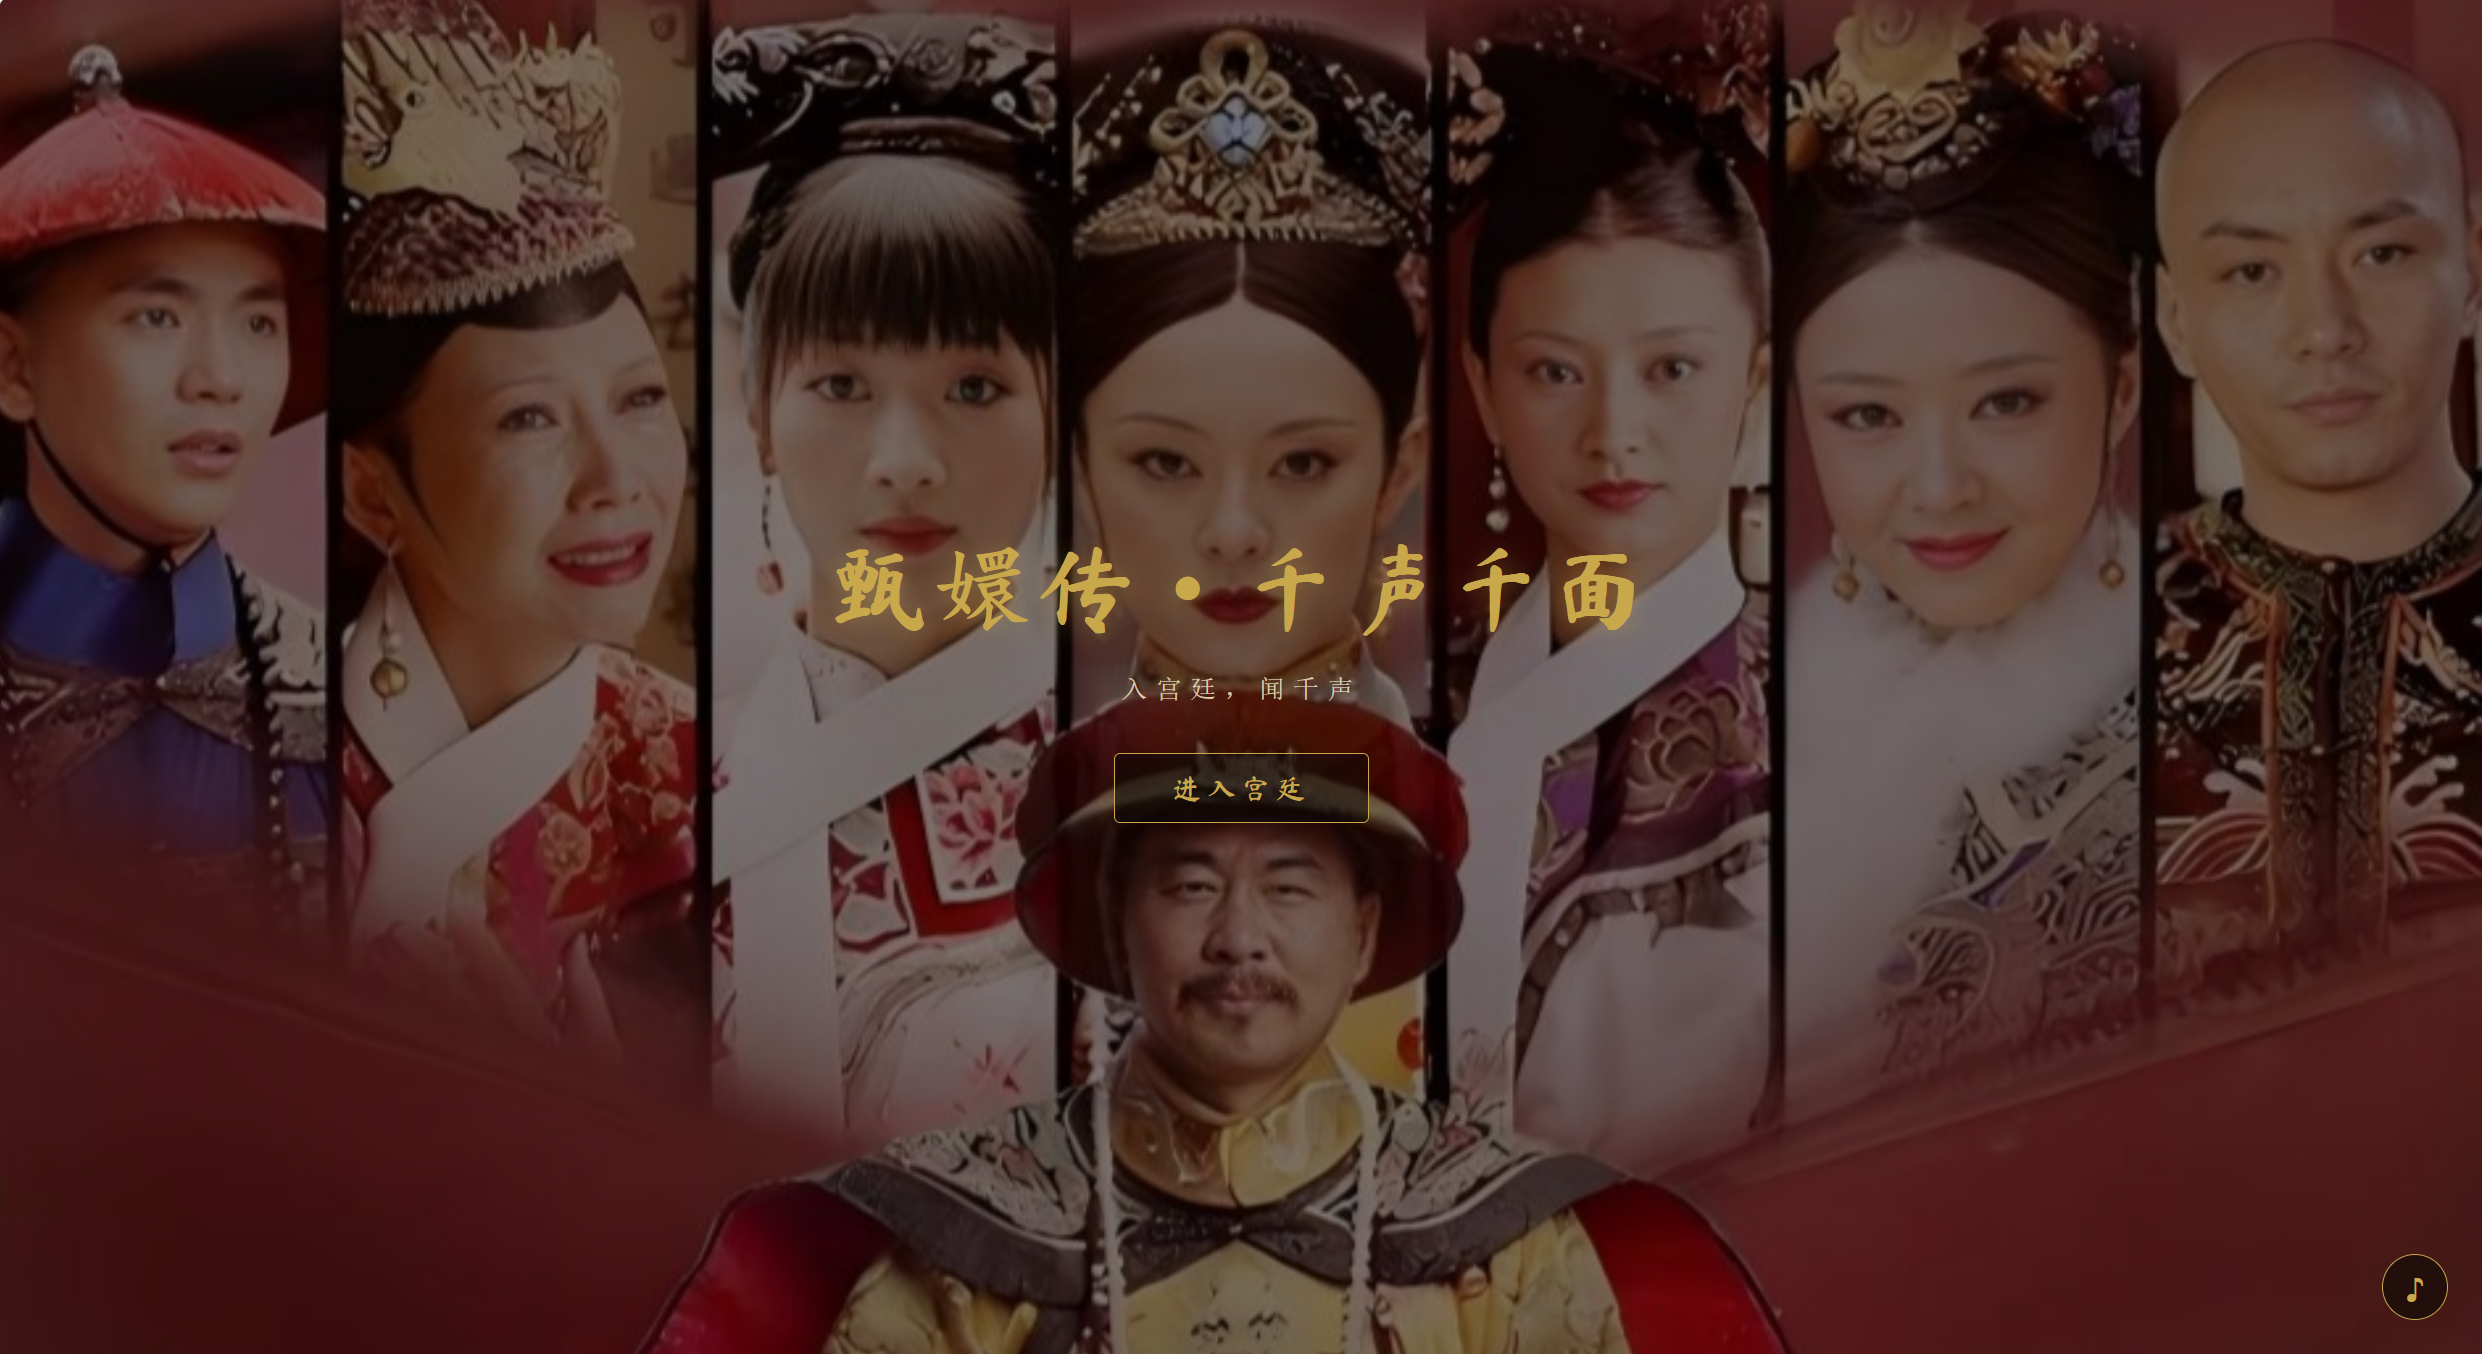
\includegraphics[width=0.85\textwidth]{figures/ui_homepage.png}
\caption{系统主页界面}
\label{fig:ui-home}
\end{figure}

\paragraph{角色选择页（CharacterSelectPage）}
提供三种交互模式入口：\textbf{现代来客}（以现代人身份入宫对话）、\textbf{宫廷中人}（扮演剧中角色参与对话）和\textbf{即兴对话}（选择两个 AI 角色自动对戏）。选择身份后展示 14 张角色卡片，每张包含角色剧照、角色名（毛笔体）和一句经典台词。卡片具有悬停放大与金色边框高亮效果。三种模式的选择界面分别如图~\ref{fig:ui-select-modern}、图~\ref{fig:ui-select-palace}和图~\ref{fig:ui-select-duet}所示。

\begin{figure}[H]
\centering
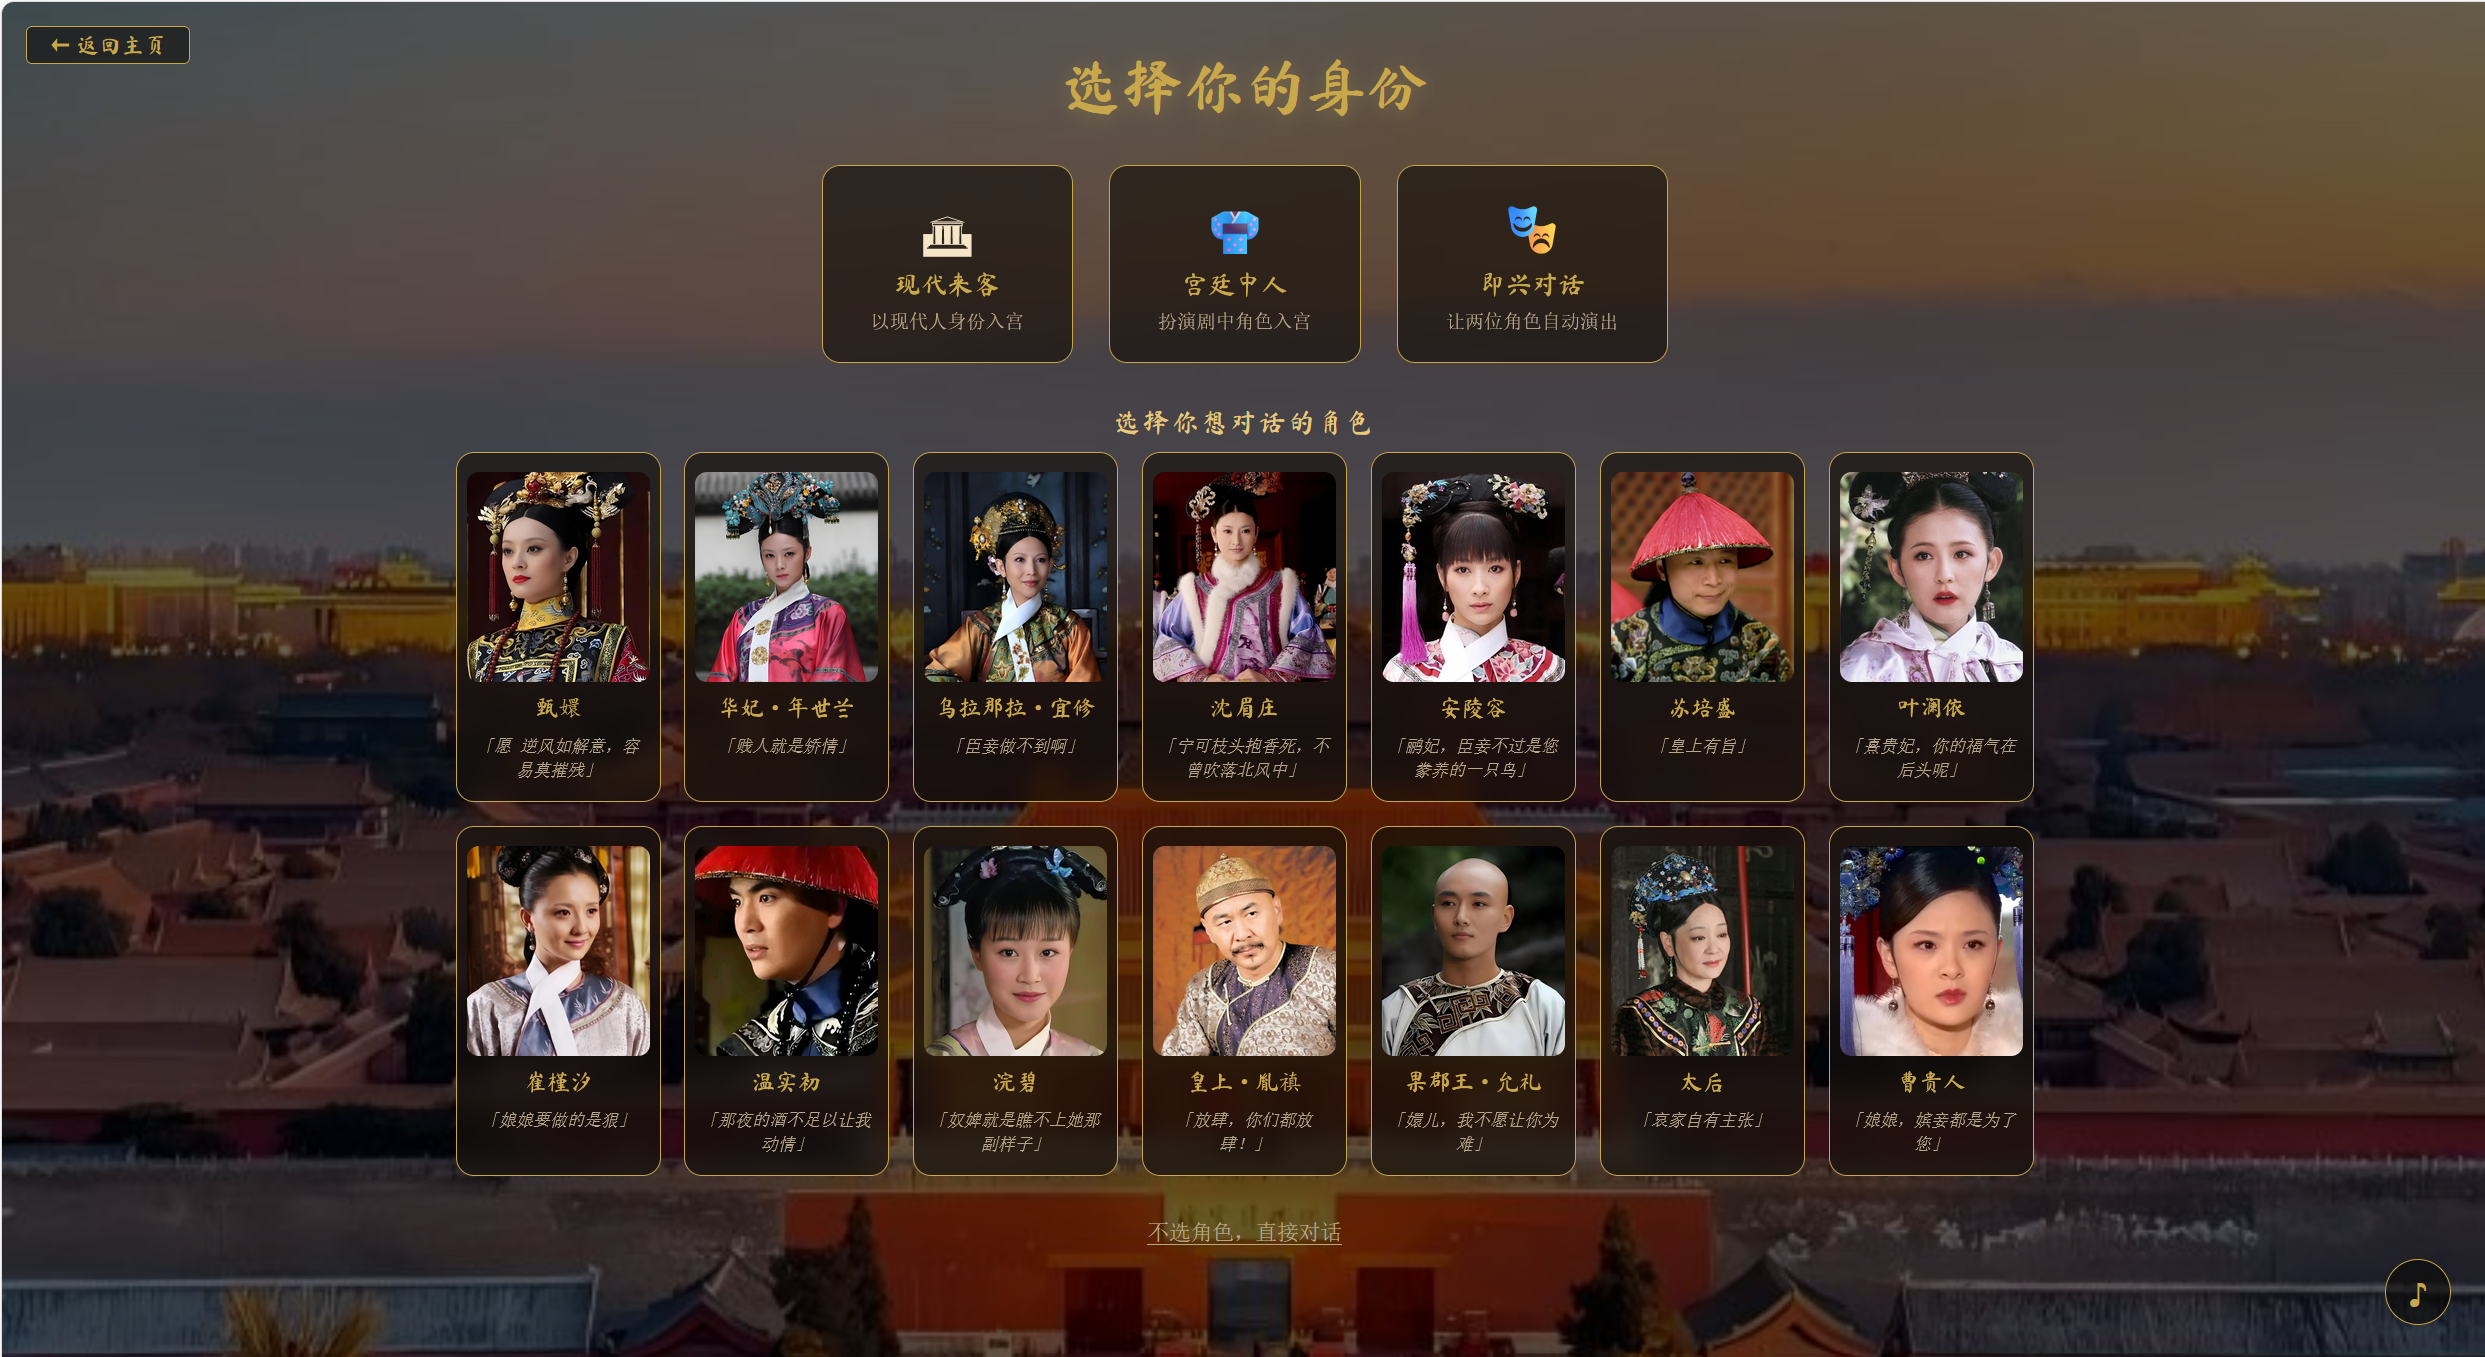
\includegraphics[width=0.85\textwidth]{figures/ui_select_modern.png}
\caption{角色选择页------现代来客模式}
\label{fig:ui-select-modern}
\end{figure}

\begin{figure}[H]
\centering
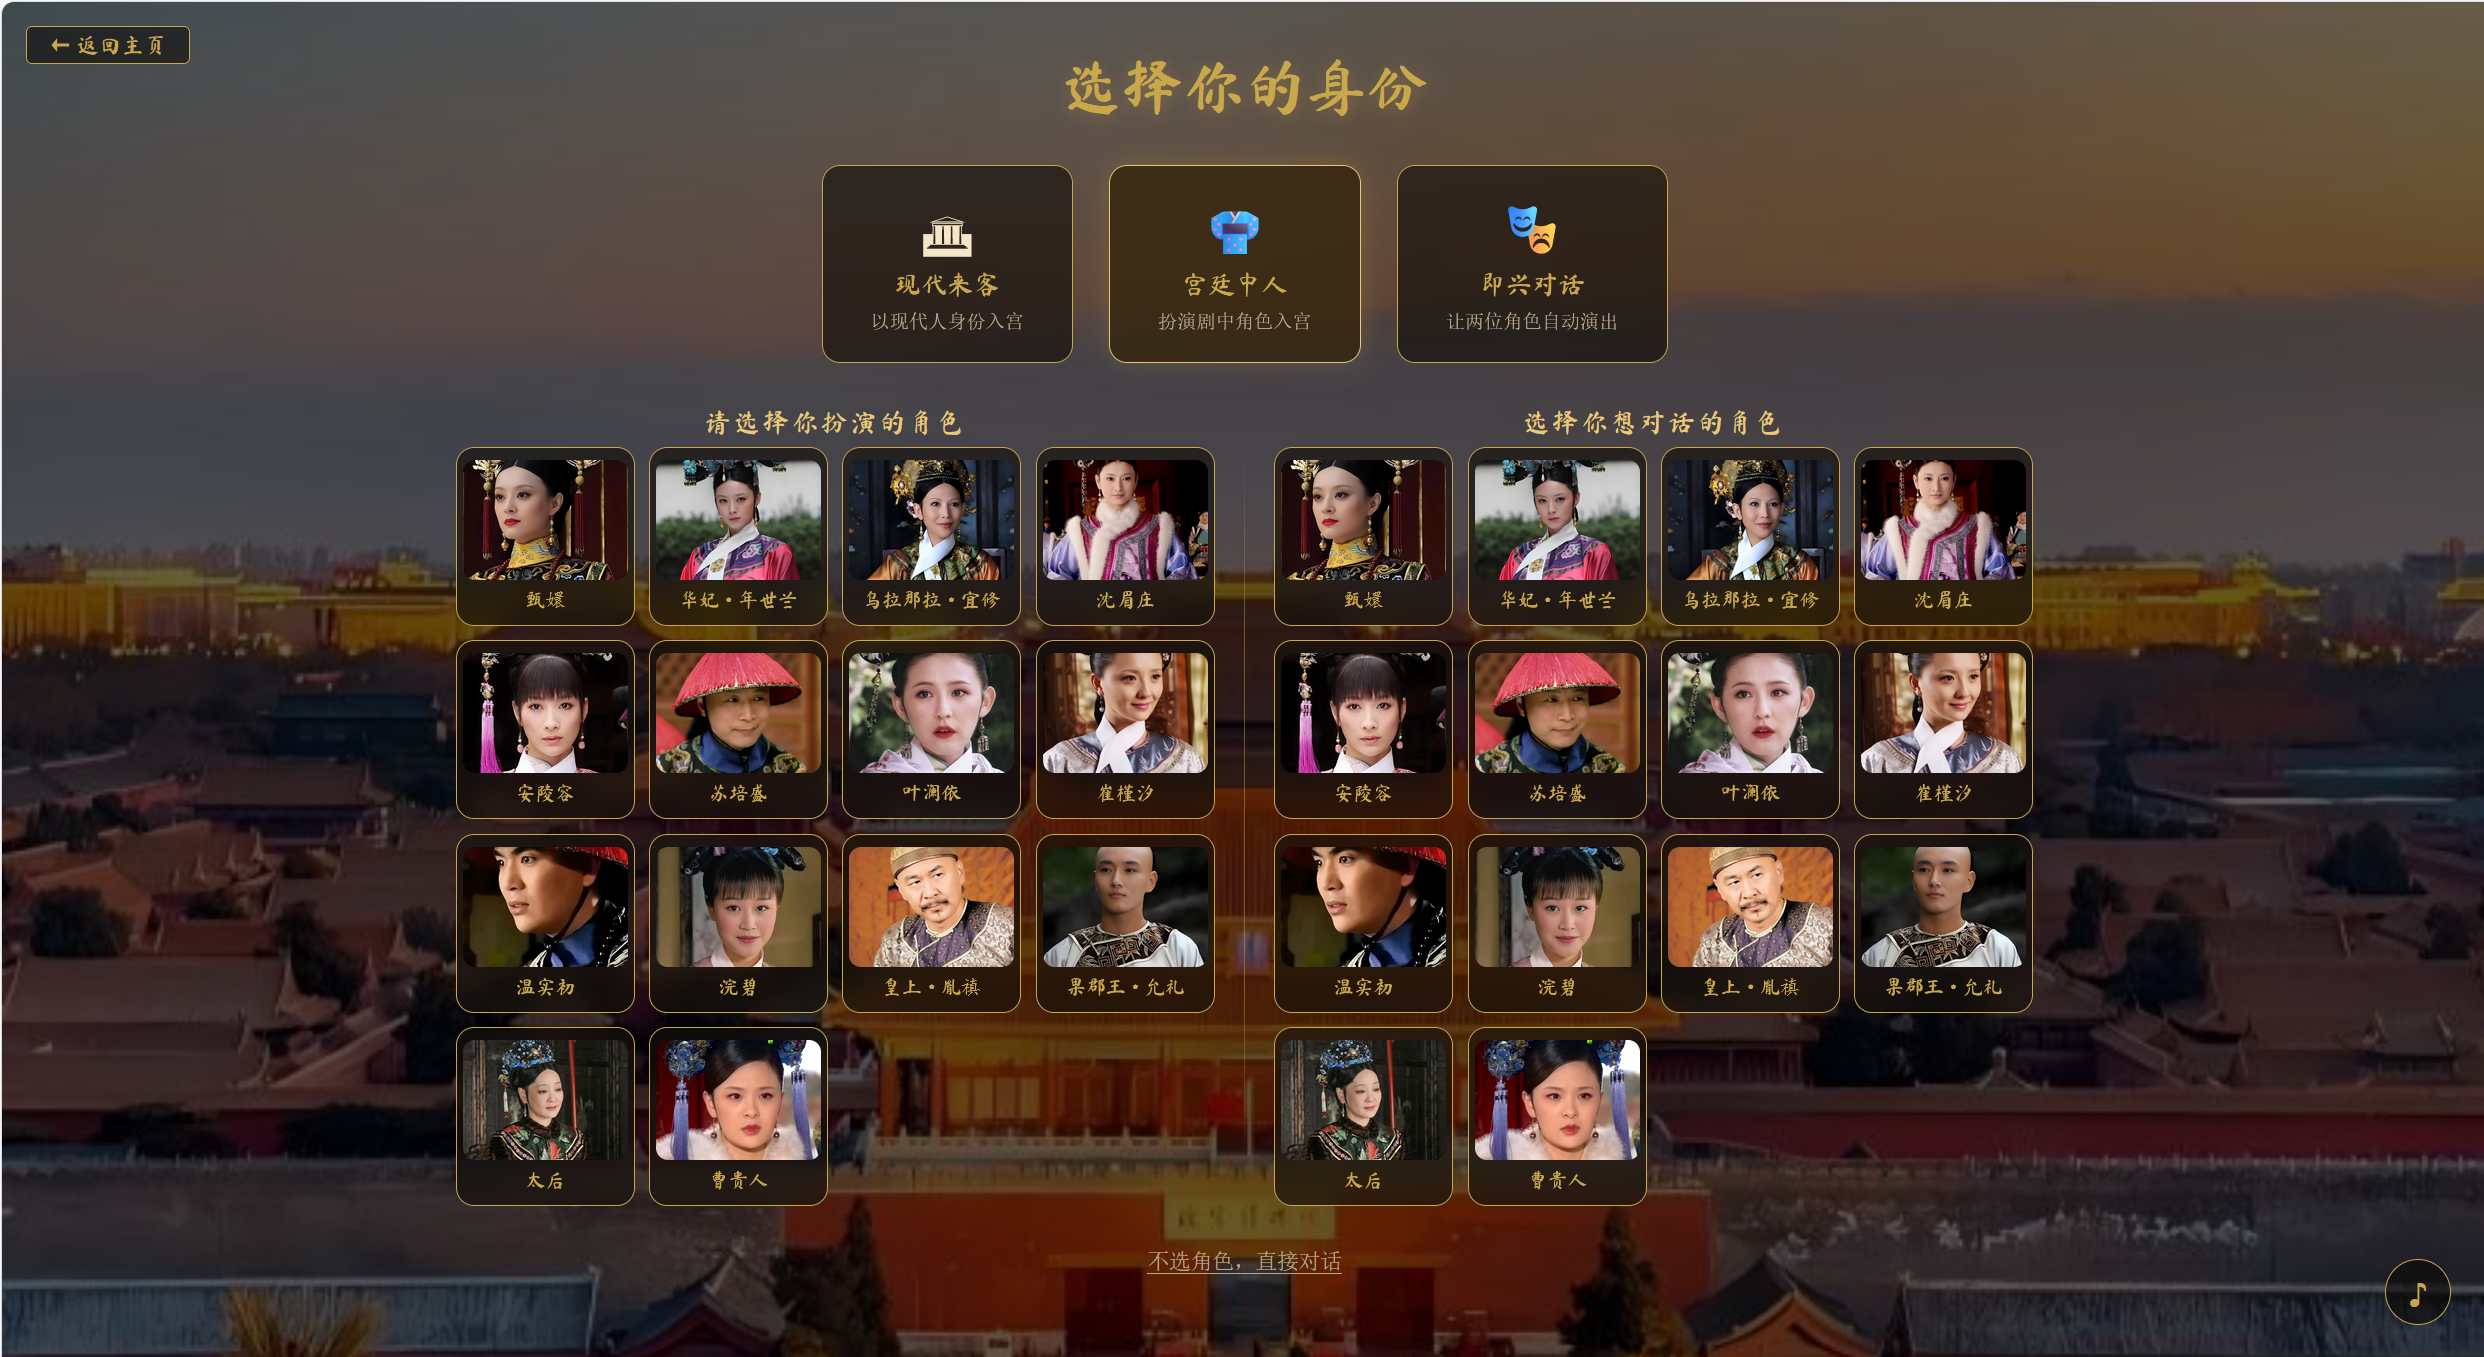
\includegraphics[width=0.85\textwidth]{figures/ui_select_palace.png}
\caption{角色选择页------宫廷中人模式（左：选择扮演角色，右：选择对话角色）}
\label{fig:ui-select-palace}
\end{figure}

\begin{figure}[H]
\centering
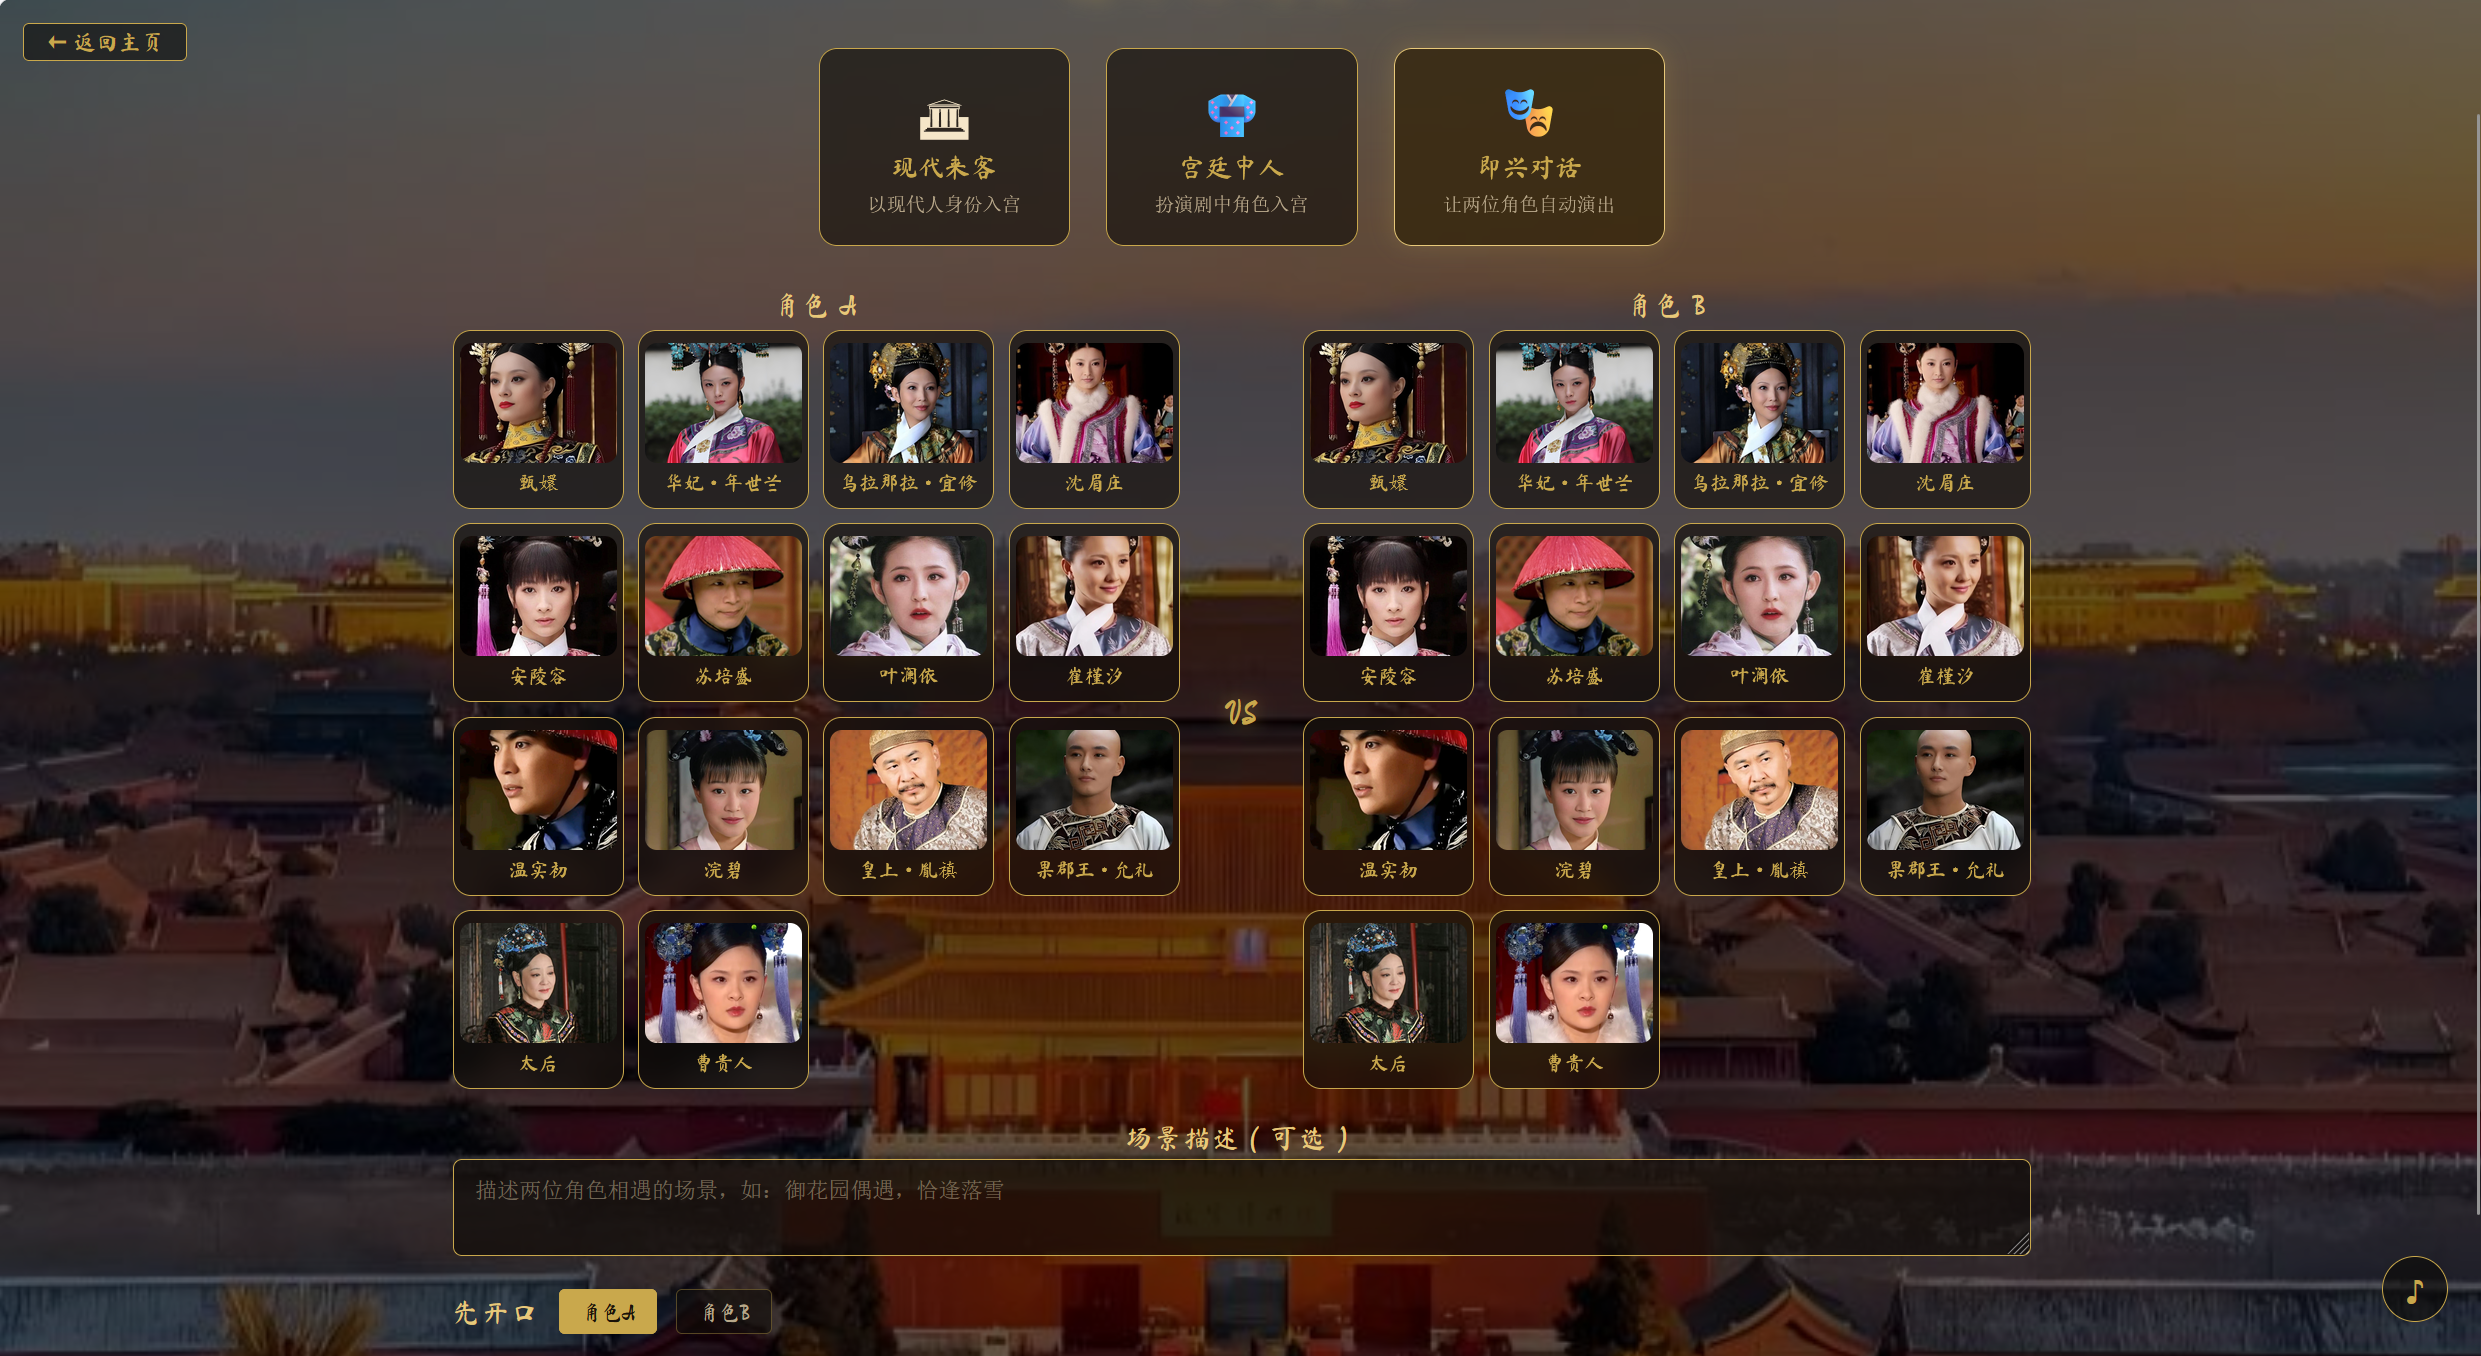
\includegraphics[width=0.85\textwidth]{figures/ui_select_duet.png}
\caption{角色选择页------即兴对话模式（左右各选一位角色 + 场景描述）}
\label{fig:ui-select-duet}
\end{figure}

\paragraph{对话页（ChatPage）}
采用左右两侧角色展示区 + 中间对话区的三栏布局（比例约 1:3:1）。两侧角色展示区显示当前角色剧照与声波动画，背景图根据对话角色动态切换。中间对话区支持文字输入、语音输入（浏览器 MediaRecorder API 录音 $\to$ ASR 识别 $\to$ 回填输入框）、快捷经典台词按钮、TTS 引擎实时切换（GPT-SoVITS / CosyVoice）和情绪手动覆盖。LLM 返回的情绪标签会触发对应视觉反馈：愤怒时背景闪烁红色遮罩，悲伤时亮度降低，喜悦时出现金色光晕。

% TODO: 补充单人对话截图
% \begin{figure}[H]
% \centering
% 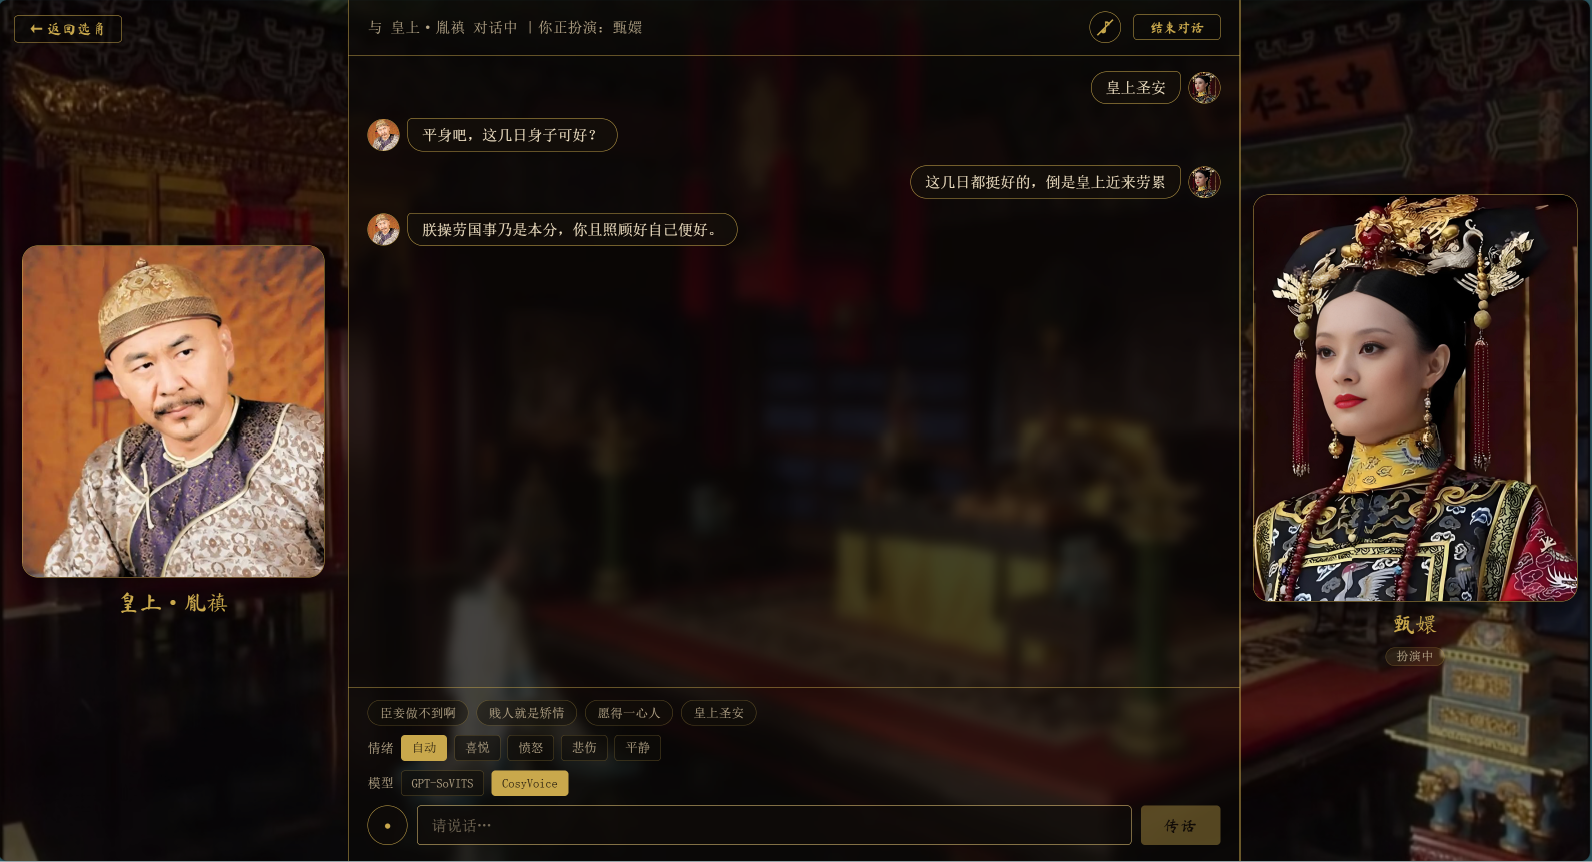
\includegraphics[width=0.85\textwidth]{figures/ui_chat.png}
% \caption{单人智能对话界面}
% \label{fig:ui-chat}
% \end{figure}

点击结束对话后弹出总结卡片，包含角色态度评价和古风总结语，支持通过 html2canvas 一键导出 PNG。

% TODO: 补充对话总结截图
% \begin{figure}[H]
% \centering
% 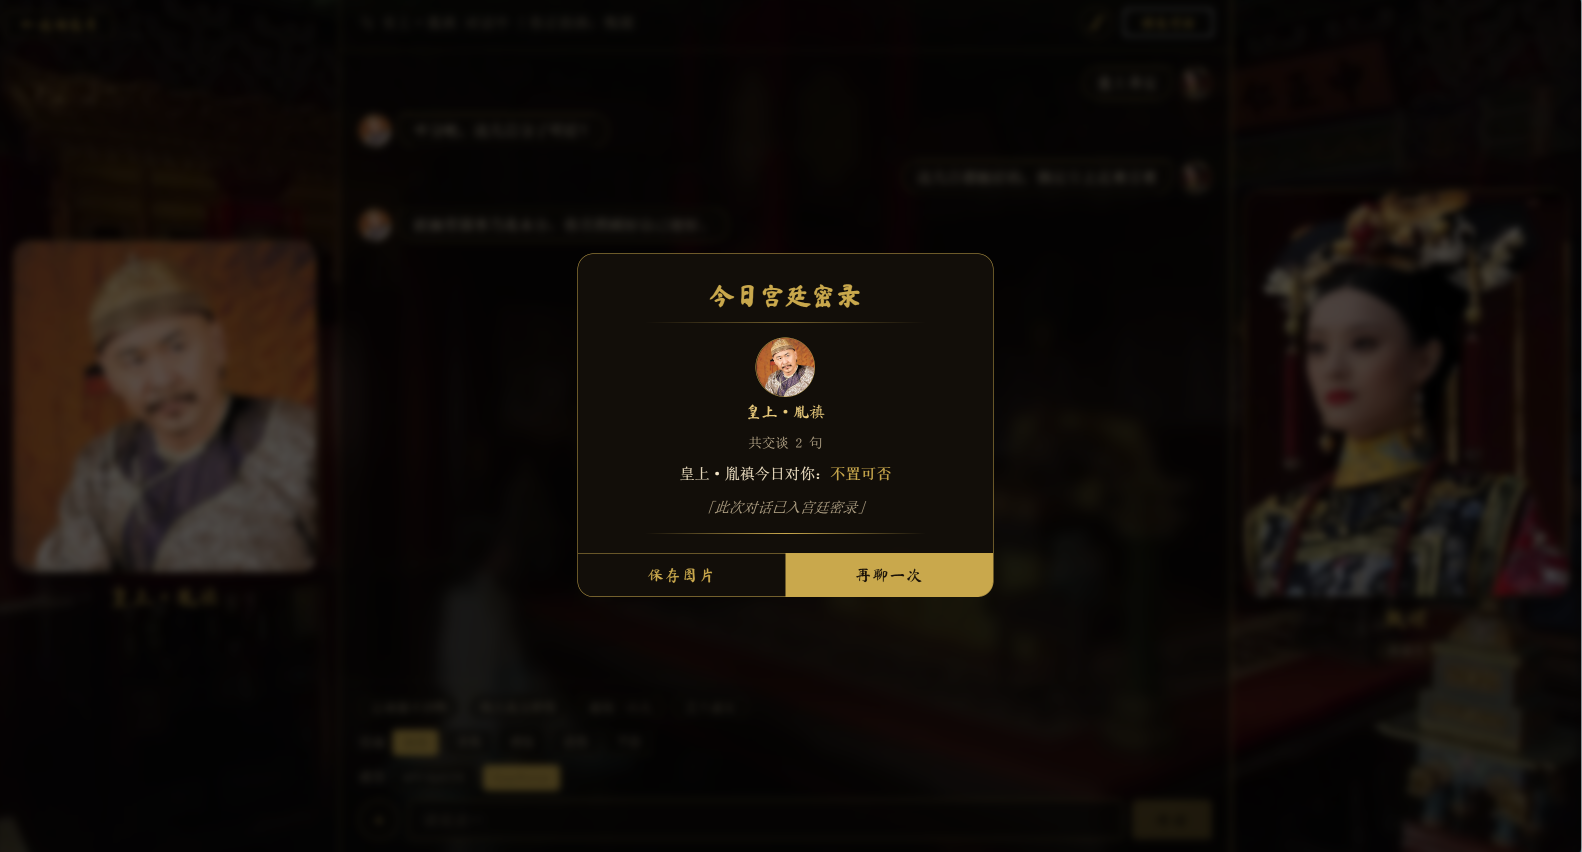
\includegraphics[width=0.5\textwidth]{figures/ui_summary.png}
% \caption{对话总结卡片}
% \label{fig:ui-summary}
% \end{figure}

\paragraph{即兴对话页（DuetPage）}
用户选择两个角色并设定场景后，两个 AI 角色自动交替对话，用户全程旁观。后端循环调用 LLM 生成回复并通过 SSE 逐轮推送文本与合成音频，前端使用 Web Audio API 按序排队播放，形成即兴对戏效果。用户可随时点击停止按钮中断对话。

% TODO: 补充双人即兴对话截图
% \begin{figure}[H]
% \centering
% 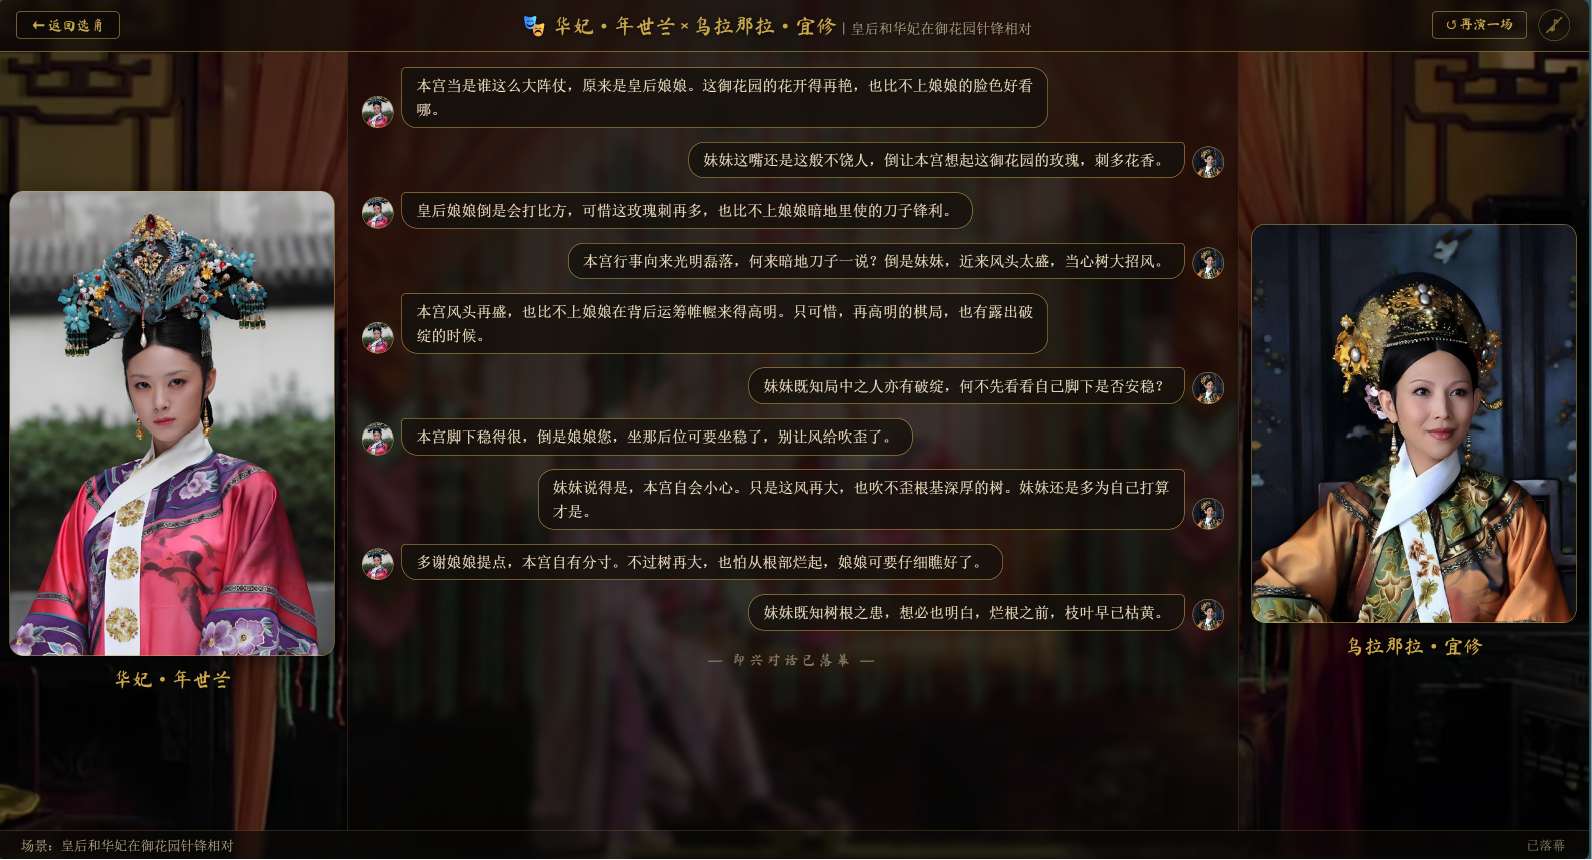
\includegraphics[width=0.85\textwidth]{figures/ui_duet.png}
% \caption{双人即兴对话界面}
% \label{fig:ui-duet}
% \end{figure}

\subsubsection{流式 TTS 链路}

CosyVoice 引擎支持流式语音合成，系统实现了完整的 SSE 流式播放链路，如图~\ref{fig:stream-tts}所示。

\begin{figure}[H]
\centering
\begin{tikzpicture}[node distance=1.6cm, auto, scale=0.82, every node/.style={transform shape}]

    \node [cterm, minimum width=5.0cm]
        (tts) {\textbf{CosyVoice TTS 服务} (\texttt{:8003}) \\ {\footnotesize AutoDL 云端，流式生成音频块}};
    \node [cproc, below=1.6cm of tts, minimum width=5.0cm]
        (mid) {\textbf{yiping-backend} (\texttt{:8000}) \\ {\footnotesize SSE 转发，每块 \texttt{\{i, audio, dur\}}}};
    \node [cproc, below=1.6cm of mid, minimum width=5.0cm]
        (web) {\textbf{前端 Web Audio API} \\ {\footnotesize 按序号 \texttt{i} 计算 startTime 排队}};
    \node [cterm, below=1.6cm of web, minimum width=5.0cm]
        (play) {\textbf{无缝顺序播放} \\ {\footnotesize 首音延迟 $\sim$1.5s，RTF 0.5$\sim$ 0.8}};

    \draw [carr] (tts) -- node[right, font=\scriptsize\color{Cdark}, xshift=2pt]{SSH 隧道} (mid);
    \draw [carr] (mid) -- node[right, font=\scriptsize\color{Cdark}, xshift=2pt]{SSE 推送} (web);
    \draw [carr] (web) -- node[right, font=\scriptsize\color{Cdark}, xshift=2pt]{AudioContext 调度} (play);

\end{tikzpicture}
\caption{CosyVoice 流式 TTS 播放链路}
\label{fig:stream-tts}
\end{figure}

流式方案相比非流式方案将首音延迟从 2$\sim$ 3 秒降低至约 1.5 秒，音频块到达后立即解码并按序号计算播放起始时间，即使网络导致块乱序也能保证播放顺序正确。

% ══════════════════════════════════════════════════════════════════════════
\section{实验结果}
\label{sec:results}

% ── 4.1 数据集构建结果 ────────────────────────────────────────────────────
\subsection{数据集构建结果}
\label{sec:result-data}

经过第~\ref{sec:data}节所述的完整数据处理流水线，成功从《甄嬛传》76 集原剧音频中自主构建了包含\textbf{14 个角色、13,605 段语音片段、总时长约 16.7 小时}的高质量中文语音数据集。最终数据分布如表~\ref{tab:data-dist} 及图~\ref{fig:pie-dist} 所示。

数据清洗效果显著（表~\ref{tab:data-clean}）：四轮过滤共剔除 2,080 段低质量数据（占比 13.3\%），其中角色过滤阶段丢弃量最大（$-$1,682 段），主要来自非目标角色片段和背景杂音；文本过滤丢弃 359 段，多为 ASR 转写异常的极短或超长文本；文本去重与音频质检仅丢弃 39 段，表明前序步骤已将绝大部分低质数据拦截，最终保留率达 86.7\%。

说话人聚类（表~\ref{tab:cluster-top15}）表现总体良好：KMeans（$n=30$）将 15,685 段的声纹特征自动聚合为 30 个簇，其中 24 个簇成功映射到 14 个剧中角色。一个值得注意的现象是，部分角色（如甄嬛）的语音片段分散在 5 个不同簇中——这是因为同一角色在不同剧情场景下的语气、情绪、语速差异较大，导致声纹特征在嵌入空间中形成了多个子簇，后期人工标注环节对这些子簇完成了跨簇合并。Top 15 簇中仅有 spk\_25（666 段、60.7 分钟）因 KMeans 错误合并了多个不同说话人的声音而最终淘汰，说明 KMeans 在多数情况下能够有效区分不同说话人，但对声纹特征接近的少数说话人存在混淆风险。

数据集按 95:5 划分训练/验证集后，导出为 CosyVoice Kaldi 格式（wav.scp / text / utt2spk / spk2utt / instruct），并进一步提取为 Parquet 格式供模型训练使用。该数据集格式通用，亦可适配 GPT-SoVITS、VITS、Fish-Speech 等主流语音合成框架。

在此全量数据集基础上，进一步手工精选了两套高质量的参考音频子集，三者构成完整的自建数据资产，如图~\ref{fig:data-assets} 所示。\textbf{Zero-shot 参考音频集}（127 条）覆盖全部 14 个角色，每角色精选 3$\sim$10 条清晰无杂音、最能代表角色典型音色的片段，用于 CosyVoice3 Zero-shot Speaker 注册（第~\ref{sec:cosyvoice}节）。\textbf{情绪参考音频集}（107 条）聚焦甄嬛、华妃、皇上、皇后四个经典角色，手工筛选其喜悦、愤怒、悲伤、平静四种真实情绪状态下语气饱满的典型片段（采集统计见表~\ref{tab:emotion-data}），用于注册 16 个情绪 Speaker。后两者均为人工逐条试听挑选，非自动筛选，确保了参考音频的高质量。

\begin{figure}[H]
\centering
\begin{tikzpicture}[node distance=1.2cm and 1.8cm, auto, scale=0.85, every node/.style={transform shape}]

    % ── 第一层：全量数据集 ────────────────────────────
    \node [aterm, minimum width=8.0cm]
        (ds) {\textbf{全量训练数据集} \\[2pt]
              {\footnotesize 76 集原剧 $\to$ 5 步流水线 $\to$ \textbf{14 角色 · 13,605 段 · 16.7 小时}}};

    % ── 第二层：两个精选子集 ──────────────────────────
    \node [aproc, below left=1.8cm and -0.8cm of ds, minimum width=4.0cm]
        (zs) {\textbf{127 条参考音频} \\[2pt]
              {\footnotesize Zero-shot Speaker 注册用} \\[1pt]
              {\footnotesize 14 角色，每角色 3--10 条} \\[1pt]
              {\footnotesize 手工挑选，优中选优}};

    \node [aproc, below right=1.8cm and -0.8cm of ds, minimum width=4.0cm]
        (emo) {\textbf{107 条情绪音频} \\[2pt]
               {\footnotesize 情绪 Speaker 注册用} \\[1pt]
               {\footnotesize 4 角色 $\times$ 4 种情绪} \\[1pt]
               {\footnotesize 手工筛选，真实情绪状态}};

    % ── 箭头 ─────────────────────────────────────────
    \draw [aarr, dashed] (ds.south) to[out=-90, in=90]
        node[left, font=\footnotesize\color{Adark}]{精选} (zs.north);
    \draw [aarr, dashed] (ds.south) to[out=-90, in=90]
        node[right, font=\footnotesize\color{Adark}]{精选} (emo.north);

    % ── 底部标注 ─────────────────────────────────────
    \node [font=\footnotesize\color{Adark}, below=0.6cm of zs, align=center]
        {$\to$ 14 基础角色声纹};
    \node [font=\footnotesize\color{Adark}, below=0.6cm of emo, align=center]
        {$\to$ 16 情绪角色声纹};

\end{tikzpicture}
\caption{自建数据资产全景：全量训练集 + 精选参考音频 + 情绪音频}
\label{fig:data-assets}
\end{figure}

\subsection{语音合成效果对比}
\label{sec:result-tts}

% [成员A+B共同撰写]
% 此部分展示两种TTS引擎的合成效果对比，包括：
%
% 1. CosyVoice3 Zero-shot vs GPT-SoVITS 微调的主观听感对比
% 2. 不同角色的音色还原度评估
% 3. 情绪Speaker方案的效果验证
% 4. 流式 vs 非流式TTS的延迟对比（首音延迟、RTF）
%
% 建议配合MOS评分表（如有）或主观评价表

\subsection{对话系统功能验证}
\label{sec:result-dialogue}

% [全组共同撰写]
% 此部分展示系统各功能模块的运行效果，包括：
%
% 1. 单人对话效果截图与分析
% 2. 双人即兴对话效果截图与分析
% 3. ASR识别准确率测试
% 4. 情绪视觉反馈与对话总结卡片展示
%
% 建议配合系统运行截图

% ══════════════════════════════════════════════════════════════════════════
\section{问题分析}
\label{sec:problems}

在项目实施过程中，团队遇到并解决了以下关键问题：

\subsection{CosyVoice3 微调过拟合}
\label{sec:prob-overfit}

如第~\ref{sec:cosyvoice}节所述，CosyVoice3-0.5B 全参数 SFT 微调在第 3 个 Epoch 出现严重过拟合，训练损失与验证损失出现显著背离（图~\ref{fig:loss-curve}）。这一问题的根本原因可归结为以下三个层面：

\textbf{(1) 梯度投票权不对等。} 14 角色联合训练时，甄嬛（29.5\%）、皇上（17.3\%）和皇后（10.6\%）三个角色合计占据约 57\% 的训练样本。模型每更新两步即有一歩被这三个角色主导，温实初（2.0\%，253 段）等小角色在整个训练过程中极少出现，其梯度信号被淹没在主导角色的梯度海洋中。

\textbf{(2) Speaker Embedding 条件信号退化。} CosyVoice3 的推理逻辑为 $\text{speaker\_embedding} + \text{text} \to \text{speech\_token}$，模型需学会根据输入声纹选择对应音色。然而，在 57\% 样本来自前三大角色的数据分布下，模型发现了一种捷径——\textit{部分忽略 Speaker Embedding，直接输出高频角色的音色特征}，因为这一策略在多数训练样本上 Loss 最低。后果是小角色的 Speaker Embedding 退化为无效信号，验证集上合成音频的音色偏向甄嬛或皇上。

\textbf{(3) 预训练表示被快速覆盖。} CosyVoice3-0.5B 的预训练权重编码了通用 TTS 能力，微调时主导角色率先改写关键表示层；小角色的少量数据无力争夺这些位置，只能附着在已被主导角色占据的表示空间之上，合成音色偏离原声是必然结果。

图~\ref{fig:overfit-chain} 将上述三条根因串联为因果链路。

\begin{figure}[H]
\centering
\begin{tikzpicture}[node distance=1.0cm and 0.6cm, auto, scale=0.82, every node/.style={transform shape}]

    \node [aterm, minimum width=2.4cm, font=\footnotesize\bfseries]
        (n1) {数据极度不均衡 \\ {\footnotesize 前3角色占57\%}};
    \node [aproc, right=of n1, minimum width=2.6cm, font=\footnotesize]
        (n2) {梯度投票权 \\ 不对等};
    \node [aproc, right=of n2, minimum width=2.6cm, font=\footnotesize]
        (n3) {Speaker Embedding \\ 条件信号退化};
    \node [aproc, right=of n3, minimum width=2.6cm, font=\footnotesize]
        (n4) {小角色音色 \\ 被大角色覆盖};
    \node [aterm, right=of n4, minimum width=2.4cm, font=\footnotesize\bfseries]
        (n5) {验证集 CV Loss \\ 反转上升};

    \draw [aarr] (n1) -- (n2);
    \draw [aarr] (n2) -- (n3);
    \draw [aarr] (n3) -- (n4);
    \draw [aarr] (n4) -- (n5);

\end{tikzpicture}
\caption{数据不均衡导致过拟合的因果链路}
\label{fig:overfit-chain}
\end{figure}

\textbf{解决方案与经验。} 果断放弃 SFT 微调路线，转向预训练模型的 Zero-shot 方案（对比分析见表~\ref{tab:sft-vs-zeroshot}）。Zero-shot 无需训练、即插即用，复用预训练模型在海量说话人数据上习得的强泛化能力，每个角色仅需 1 条 5$\sim$15 秒参考音频即可实现高保真音色克隆。经验表明：\textit{在小规模且极度不均衡的数据集上，端到端全参数微调并非最优策略；充分利用预训练模型的泛化能力的 Zero-shot 方案在音色还原度、发音清晰度和可扩展性上均具有显著优势。}

\subsection{GPT-SoVITS 训练与调优}
\label{sec:prob-gptsovits}

% [成员B负责撰写]
% 分析内容：
% - 小角色（如温实初仅20分钟数据）微调效果不稳定
% - v4与v2ProPlus版本在不同角色上表现不一，需逐角色选择最优版本
% - LoRA rank选择对过拟合-欠拟合的影响
% - 解决方案：单角色独立微调 + 双版本并行 + LoRA约束

\subsection{情绪控制与音色保真的矛盾}
\label{sec:prob-emotion}

Zero-shot 方案（第~\ref{sec:cosyvoice}节）能够完美复现角色的中性音色，但面临一个核心矛盾：如何在不损失音色保真度的前提下实现自然的情感表达？

\textbf{Instruct 控制的局限。} CosyVoice3 提供了 Instruct 控制接口，可通过文字指令驱动模型以特定情绪说话。然而实验发现，Instruct 方式在施加情绪控制的同时，会对声纹嵌入的表示空间产生干扰，导致输出音色偏离参考说话人的原始特征——\textit{情绪控制与音色保真构成一对矛盾，难以兼顾。}GPT-SoVITS 引擎面临类似困境：其本身不支持稳定的情绪参数直接输入，只能通过替换参考音频来间接影响输出语气（参见第~\ref{sec:prob-gptsovits}节）。

\textbf{情绪 Speaker 方案。} 为解决上述矛盾，提出了一种创新的\textbf{情绪 Speaker}方案：不依赖 Instruct 指令或参数化情绪控制，而是从 76 集原剧音频中手工筛选角色在真实情绪状态下的台词片段，将这些情绪音频本身作为独立的 Zero-shot Speaker 注册（采集统计见表~\ref{tab:emotion-data}）。推理时，根据前端传入的 \texttt{character\_id} 和 \texttt{emotion} 字段查表路由到对应的情绪 Speaker，本质上是使用该角色在\textit{真实情绪状态}下的声纹特征进行语音合成——走纯 Zero-shot 路径，因此\textbf{音色完全不丢失}。

\textbf{方案效果。} 该方案有效解决了情绪控制与音色保真之间的矛盾：在喜悦、愤怒、悲伤、平静四种情绪上，合成音频的语气自然贴近剧中角色的真实情绪表达，同时保持了与中性 Speaker 一致的音色还原度。在 CosyVoice3 引擎上，该方案已成为系统默认的情绪控制策略。在 GPT-SoVITS 引擎上，同样采用情绪参考音频替代单一中性参考音频的方式实现情绪路由，但在音色一致性上略逊于 CosyVoice3 的 Zero-shot 方案（详见第~\ref{sec:prob-gptsovits}节）。


% ══════════════════════════════════════════════════════════════════════════
\section{总结与展望}
\label{sec:conclusion}

\subsection{项目成果}

本项目成功构建了《甄嬛传》多角色语音对话系统，主要成果如下：

\begin{itemize}[leftmargin=*]
    \item 自主构建了包含 14 个角色、13,605 段语音片段、总时长约 16.7 小时的高质量中文语音数据集。
    \item 实现了 CosyVoice3 Zero-shot（30 个 Speaker）与 GPT-SoVITS 微调（28 组权重）的双引擎语音合成。
    \item 创新性地提出了\textbf{情绪 Speaker}方案，通过 107 段手工采集的真实情绪音频实现了 4 种情感语音合成，有效解决了情绪控制与音色保真的矛盾。
    \item 实现了单人智能对话与双人即兴对戏两种交互模式，支持流式语音播放，首音延迟约 1.5 秒。
    \item 构建了完整的前后端系统，包含古风宫廷风格 UI、FastAPI 中间层和云端 GPU 服务。
\end{itemize}

\subsection{未来展望}

\begin{itemize}[leftmargin=*]
    \item 扩充更多角色（如端妃、敬妃、流朱等）和更多情绪类别。
    \item 探索更高效的微调策略（如单角色独立微调 + LoRA），解决数据不均衡下的过拟合问题。
    \item 引入数字人技术（SadTalker / MuseTalk），在算力允许时实现角色视频对话。
\end{itemize}

% ══════════════════════════════════════════════════════════════════════════
% 参考文献（后续在正文中用到时再逐条添加）
% ══════════════════════════════════════════════════════════════════════════
\newpage
\phantomsection
\addcontentsline{toc}{section}{参考文献}

\begin{thebibliography}{99}

\bibitem{du2025cosyvoice3} Du Z, Chen S, Ma Z, et al. CosyVoice 3: Towards Ultra-High-Fidelity Speech Synthesis with Large Language Models[C]. arXiv, 2025.
\bibitem{funasr} Gao Z, Li Z, Wang J, et al. FunASR: A Fundamental End-to-End Speech Recognition Toolkit[C]. Interspeech, 2023.
\bibitem{3d-speaker} Chen Z, Yao Y, Zheng S, et al. 3D-Speaker: A Multi-modal Open-source Toolkit for Speaker Verification and Diarization[C]. arXiv:2306.15354, 2023.
\bibitem{uvr5} Anjok07. Ultimate Vocal Remover GUI v5[EB/OL]. \texttt{https://github.com/Anjok07/ultimatevocalremovergui}, 2023.
\bibitem{defossez2021demucs} Défossez A. Hybrid Spectrogram and Waveform Source Separation[C]. ISMIR 2021 Workshop on Music Source Separation, 2021.
\bibitem{sklearn} Pedregosa F, Varoquaux G, Gramfort A, et al. Scikit-learn: Machine Learning in Python[J]. Journal of Machine Learning Research, 2011, 12: 2825--2830.
\bibitem{gptsovits} RVC-Boss. GPT-SoVITS[EB/OL]. \texttt{https://github.com/RVC-Boss/GPT-SoVITS}, 2024.
\bibitem{faster-whisper} SYSTRAN. faster-whisper[EB/OL]. \texttt{https://github.com/SYSTRAN/faster-whisper}, 2023.

\end{thebibliography}

% ══════════════════════════════════════════════════════════════════════════
% 附录
% ══════════════════════════════════════════════════════════════════════════
\newpage
\phantomsection
\addcontentsline{toc}{section}{附录\;A\;\; 网盘数据说明}
\section*{附录 A \quad 网盘数据说明}

本项目构建的数据集与模型权重因体积较大，统一上传至百度网盘，不随论文代码仓库分发。

\begin{flushleft}
\textbf{链接}：\url{https://pan.baidu.com/s/1\_uacMyl9y5YvrWsh77Mtww?pwd=kcs7} \\
\textbf{提取码}：\texttt{kcs7}
\end{flushleft}

网盘目录 \texttt{甄嬛传千声千面\_\,相关数据/} 包含以下内容：

\begin{table}[H]
\centering
\caption{网盘数据目录一览}
\label{tab:pan-data}
\renewcommand{\arraystretch}{1.4}
\begin{tabularx}{\textwidth}{p{4.5cm}p{4.0cm}X}
\toprule
\textbf{目录/文件} & \textbf{内容} & \textbf{使用方式} \\
\midrule
\rowcolor{Agray} \texttt{zero\_shot\_data/} & 127 条参考音频（14 角色）  & Zero-shot Speaker 注册用（第~\ref{sec:cosyvoice}节） \\
\texttt{emotion\_examples/}  & 107 条情绪音频（4 角色 $\times$ 4 情绪） & 情绪 Speaker 注册用（第~\ref{sec:cosyvoice}节） \\
\rowcolor{Agray} \texttt{甄嬛传14人物数据.tar} & 13,605 段 WAV + Kaldi 元数据 & Pipeline 最终产出，可用于重训练或转其他格式（第~\ref{sec:data}节） \\
\texttt{gpt\_sovits finetune\_data/} & GPT-SoVITS 微调清单与脚本 & 14 角色 train/dev 列表及批量微调脚本 \\
\rowcolor{Agray} \texttt{exp\_GPTSoVITS\_weights/} & GPT-SoVITS 14 角色权重 & v4 + v2ProPlus 两套权重（第~\ref{sec:gptsovits}节） \\
\texttt{exp\_zhenhuan\_llm.tar} & CosyVoice3-0.5B 微调权重（12 GB）& Epoch 0$\sim$4 checkpoint（第~\ref{sec:cosyvoice}节） \\
\bottomrule
\end{tabularx}
\end{table}

\textbf{数据集详情}：经过第~\ref{sec:data}节所述的全流程处理后，最终数据集包含 14 个角色、共 13,605 段语音片段（16 kHz 单声道 PCM WAV），总时长约 1,005 分钟（16.7 小时），每段 2$\sim$15 秒，按 95:5 划分为训练/验证集。数据格式为 CosyVoice Kaldi 标准（wav.scp / text / utt2spk / spk2utt / instruct），亦可通过脚本转换为 GPT-SoVITS、VITS、Fish-Speech 等框架的输入格式（脚本参见项目仓库 \texttt{siting\_data\_prepare/scripts/}）。

\textbf{模型权重说明}：CosyVoice3 SFT 微调权重因过拟合问题最终未被系统采用（分析见第~\ref{sec:prob-overfit}节），保留供后续研究参考。系统实际运行使用的是 CosyVoice3 Zero-shot 方案（预训练权重）和 GPT-SoVITS 微调权重，后者为系统备用 TTS 引擎。

\newpage
\phantomsection
\addcontentsline{toc}{section}{附录\;B\;\; 小组成员分工}
\section*{附录 B \quad 小组成员分工}

\begin{table}[H]
\centering
\renewcommand{\arraystretch}{1.5}
\begin{tabularx}{\textwidth}{p{2.0cm}p{2.0cm}p{1.8cm}X}
\toprule
\textbf{成员} & \textbf{姓名} & \textbf{学号} & \textbf{负责内容} \\
\midrule
成员A & 李思婷 & 2023212061 &
\begin{minipage}[t]{\linewidth}
\begin{itemize}[leftmargin=*, nosep, topsep=0pt]
    \item 数据集构建：76集原剧音频处理全流程（人声分离→VAD切分→ASR转写→声纹聚类→人工标注→数据清洗）
    \item CosyVoice3-0.5B 微调实验与过拟合分析
    \item CosyVoice3 Zero-shot 方案：14角色Speaker注册
    \item 情绪Speaker创新方案：手工采集107段真实情绪音频，注册16个情绪Speaker
\end{itemize}
\end{minipage} \\
\midrule
成员B & 张笑 & 2023212062 &
\begin{minipage}[t]{\linewidth}
\begin{itemize}[leftmargin=*, nosep, topsep=0pt]
    \item GPT-SoVITS 微调：14角色$\times$2版本=28组独立权重训练
    \item ASR 模块：faster-whisper-small 部署与配置
    \item LLM 对话模块：角色人设Prompt设计、单人对话与双人即兴对话生成
    \item GPT-SoVITS 服务端部署与情绪参考音频路由
    \item 参与情绪音频采集与标注
\end{itemize}
\end{minipage} \\
\midrule
成员C & 黄艺平 & 2023212179 &
\begin{minipage}[t]{\linewidth}
\begin{itemize}[leftmargin=*, nosep, topsep=0pt]
    \item 前端设计：React古风宫廷UI（主页、角色选择、对话、即兴对话四页面）
    \item 视觉素材采集：12张角色剧照、11张场景背景图、1首背景音乐
    \item yiping-backend 中间层：统一API网关、云端服务路由与对接
    \item 流式TTS链路集成：SSE + Web Audio API 排队播放
\end{itemize}
\end{minipage} \\
\bottomrule
\end{tabularx}
\caption{小组成员分工详情}
\label{tab:team}
\end{table}

\end{document}
